%--------------------------------------------------------------------------------------------------
% ips-phd-thesis-eng-ieee.tex v1.2 (see the end of the file for modification history)
% Version 1.2 released 2015/04/13
%
% A template for creating a PhD thesis in English using the APA 6th edition reference formatting
% with several accompanying files.
% By Tea Tušar <tea.tusar@ijs.si>
%
% IMPORTANT NOTE: Biber must be used as the backhand for processing bibliographies, not bibtex!
%
% To compile this template, you need to run the following sequence of commands:
% 1. pdflatex  ips-phd-thesis-eng-ieee
% 2. biber     ips-phd-thesis-eng-ieee
% 3. makeindex ips-phd-thesis-eng-ieee (optional, if you want an index)
% 4. pdflatex  ips-phd-thesis-eng-ieee
% 5. pdflatex  ips-phd-thesis-eng-ieee
%--------------------------------------------------------------------------------------------------
\documentclass[phd,eng,ieee]{ipsthesis}
%
%--------------------------------------------------------------------------------------------------
%
% PREAMBULE
%--------------------------------------------------------------------------------------------------
%
% Files with bibliographies
\addbibresource{references.bib}
%
% Define here all other packages and commands you need for your thesis, for example:
\usepackage{color}
\usepackage{longtable}

\usepackage{algorithmic}
\usepackage{subcaption}
\usepackage{graphicx}

\newcommand{\RR}{\mathbb{R}}
\newcommand{\X}{\mathbb{X}}
\newcommand{\Y}{\mathbb{Y}}
\newcommand{\NN}{\mathbb{N}}
\newcommand{\sym}{\mathbb{S}}
\newcommand{\dataset}{{\cal D}}
\newcommand{\fracpartial}[2]{\frac{\partial #1}{\partial  #2}}
\newcommand\Prefix[3]{\vphantom{#3}#1#2#3}


%\usepackage{theorem}
\newtheorem{lemma}[theorem]{Lemma}
\newtheorem{proposition}[theorem]{Proposition}
\newtheorem{corollary}[theorem]{Corollary}
\newtheorem{assumption}[theorem]{Assumption}
\newtheorem{conjecture}[theorem]{Conjecture}

\newenvironment{notation}[1][Notation]{\begin{trivlist}
\item[\hskip \labelsep {\bfseries #1}]}{\end{trivlist}}

\newcommand{\abs}[1]{\lvert#1\rvert}
\newcommand{\norm}[1]{\lVert#1\rVert}



%--------------------------------------------------------------------------------------------------
%
% DOCUMENT
%--------------------------------------------------------------------------------------------------
\begin{document}
%--------------------------------------------------------------------------------------------------
%
% The cover page and spine are created separately using two .doc files provided by IPS.
%--------------------------------------------------------------------------------------------------
%
% FRONT MATTER
%--------------------------------------------------------------------------------------------------
%
\frontmatter
%
\selectlanguage{american}
\pagestyle{fancy}
%
% Title pages
%--------------------------------------------------------------------------------------------------
%
% INPUT FOR THE TITLE PAGES
%--------------------------------------------------------------------------------------------------
%
% Author
\author{Jan Rupnik}
%
% Title in English (use \protect\\ instead of \\ to create a line break)
\titleEnglish{Multi-View Canonical Correlation Analysis}
%
% Title in Slovene (use \protect\\ instead of \\ to create a line break)
\titleSlovene{Kanonična Korelacijska Analiza  za Več Množic Spremenljivk}
%
% Supervisor (title and name, affiliation)
\supervisorOne{Prof.\ Dunja Mladenić}{Artificial Intelligence Laboratory, Jožef Stefan Institute, Ljubljana, Slovenia}
%
% Co-supervisor (title and name, affiliation), optional
\supervisorTwo{Prof.\ John Shawe-Taylor}{Department of Computer Science, University College London, Gower Street, London WC1E 6BT, United Kingdom}
%
% Co-supervisor (title and name, affiliation), optional
%\supervisorThree{Prof.\ Name Surname3}{Institution3, Place, Country}
%
% Evaluation board chairman (title and name, affiliation)
\evaluationBoardChairman{Prof.\ Name SurnameA}{InstitutionA, Place, Country}
%
% Evaluation board member #1 (title and name, affiliation)
\evaluationBoardMemberOne{Prof.\ Name SurnameB}{InstitutionB, Place, Country}
%
% Evaluation board member #2 (title and name, affiliation)
\evaluationBoardMemberTwo{Prof.\ Name SurnameC}{InstitutionC, Place, Country}
%
% Date
\month{December}
\year{2015}
%
\maketitle 
%
% Dedication (optional)
%--------------------------------------------------------------------------------------------------
%
% INPUT FOR THE DEDICATION
%--------------------------------------------------------------------------------------------------
\dedication{To ...}
\makededication 
%
% Acknowledgments
%--------------------------------------------------------------------------------------------------
%
\chapter*{Acknowledgments}
\pdfbookmark[0]{Acknowledgments}{Acknowledgments}
%--------------------------------------------------------------------------------------------------

I would like to express great appreciation to my PhD supervisor Prof. Dunja
Mladenić and co-supervisor Prof. John Shawe-Taylor for their guidance and advice
throughout my studies. Special thanks go to Primož Škraba for his invaluable advice and contributions to my work.
I would also like to thank Marko Grobelnik for providing inspiration and encouragement for my research work.

Assistance provided by my collaborators Andrej Muhič, Blaž Fortuna, Gregor Leban
and Sabrina Guettes was greatly appreciated. It was my great pleasure working with you.
I would also like to thank my friends from UCL: Tom Diethe, David Roi Hardoon and Zakria Hussain
for great company and discussions during my visits to UCL.

My gratitude goes to the members of my doctoral committee, Prof. Nada Lavrač, Prof.
Bor Plestenjak and Prof. Nicolò Cesa-Bianchi, for their valuable comments and
remarks.

Finally, I wish to thank Zala, my parents Darja and Erik and my sister Nika
for their support and encouragement.

\rule{0.5\textwidth}{.4pt}

The author gratefully acknowledges funding by the projects
SMART (IST-5-033917-STP), X-LIKE (ICT-257790-STREP), MultilingualWeb (PSP-2009.5.2 Agr.\# 250500),
TransLectures (FP7-ICT-2011-7), PlanetData (ICT-257641-NoE), RENDER (ICT-257790-STREP), XLime (FP7-ICT-611346),
and META-NET (ICT-249119-NoE). 
%
% English abstract
%--------------------------------------------------------------------------------------------------
% 
\chapter*{Abstract}
\pdfbookmark[0]{Abstract}{Abstract}
%--------------------------------------------------------------------------------------------------

The English abstract should not take up more than one page.
%
% Slovene abstract, switch to slovene
\selectlanguage{slovene}
%--------------------------------------------------------------------------------------------------
%
\chapter*{Povzetek}
\pdfbookmark[0]{Povzetek}{Povzetek}
%--------------------------------------------------------------------------------------------------

Metode, ki temeljijo na matrični faktorizaciji, predstavljajo pomemben pristop k analizi vzorcev
in podatkovnemu rudarjenju. Naloge, ki jih lahko prevedemo na matrične razcepe, vključujejo izbiranje 
s sodelovanjem (ang. {collaborative filtering}), vstavljanje manjkajočih podatkov (ang. \emph{missing data imputation}), 
zmanjševanje dimenzij (ang. \emph{dimensionality reduction}, odstranjevanje šuma (ang. \emph{denoising}, vizualizacija
podatkov (ang. \emph{data visualization}) in eksploratorna analiza podatkov (ang. \emph{exploratory data analysis}).

V pričujoči disertaciji se ukvarjamo z \emph{večpogledno učenjem} (ang. \emph{multiview learning}), kjer
predpostavljamo, da imamo na podatke dva ali več \emph{pogledov} (ang. \emph{views}), kar konkretneje
pomeni, da imamo za vsako podatkovno instanco na voljo dve ali več množic značilk (ang. \emph{feature sets}),
ki predstavljajo različne poglede na nek objekt. Primer podatkovne množice primerne za večpogledno učenje
je množice parov slik in tekstovnih opisov, ki ustrezajo slikam. Predpostavljamo, da lahko slike in besedila
predstavimo kot objekte v dveh vektorskih prostorih, katerih dimenzije ustrezajo značilkam za analizo
slik oziroma besedil. V tem primeru iščemo vzorce (predstavljene kot funkcionale) v prostoru slik
in tekstovnem prostoru, ki so paroma močno povezani (na primer visoko korelirani vzdolž učne množice).

Kanonična Korelacijks Analiza (KKA) predstavlja enega izmed najpomembnejših pristopov za analizo
podatkov, kjer sta na voljo dva pogleda oziroma dve množici spremenjlivk. V pričujočem delu
preučujemo dve posplošitvi metode KKA za analizo poljubnega števila množic značilk: metoda
Vsote Korelacij (VKOR) (ang. \emph{Sum Of Correlations}) metode Vsote Kvadratov Korelacij (VKKOR).
Optimizacijski problem povezan s posplošitvijo VKOR se pojavi tudi v drugih problemih, med drugim
v teoriji regulacije, nalogah slepega ločevanja signalov (ang. \emph{Blind Source Signal Separation})
in analizi meritev funkcionalne magnetne resonance na skupinah subjektov.

Omenjeni posplošitvi VKOR in VKKOR preučimo z večih vidikov. Prvi prispevek k znanosti predstavlja
dokazano konvergentni algoritem za iskanje večih množic nelinearnih vzorcev, 
ki temelji na iterativni metodi za reševanje multivariatnih problemov lastnih vrednosti (ang. 
\emph{multivariate eigenvalue problems}). Dokažemo, da je problem KKRO v splošnem NP-težek,
kar nas privede do analize konveksne relaksacije in prevedbe na optimizacijsko nalogo
semidefinitnega programiranja (SDP) (ang. \emph{Semidefinite Programming}). Na podlagi
SDP formulacije predstavimo številne nove spodnje meje za vrednost globalno optimalne
rešitve. Čeprav so meje izračunjlive v polinomskem času, je njihov izračun v praksi
lahko težaven. Zato predstavimo pristop, ki temelji na zmanjšanju števila spremenljivk s
pomočjo naključnih projekcij. Predstavimo tudi aplikacijo posplošitev KKA na problemu
učenja jezikovno neodvisne mere podobnosti, kjer naletimo na problem manjkajočih
učnih podatkov. Pokažemo, da določena struktura manjkajočih podatkov pripelje do
poenostavitve optimizacijskega problema KKRO, ki ga prevedemo računsko manj zahteven 
problem lastnih vrednosti. Pokažemo, kako lahko uporabimo jezikovno neodvisno mero podobnosti
za medjezično povezovanje gruč dokumentov. Pristop uporabimo v sistemu za globalno analizo
tokov novic v večih jezikih.



\selectlanguage{american}
%
% Contents
\maketoc
%
% List of figures (required if the thesis contains figures)
\makelof
%
% List of tables (required if the thesis contains tables)
\makelot
%
% List of algorithms (required if the thesis contains algorithms)
\makeloa
%
% Abbreviations (optional)
%--------------------------------------------------------------------------------------------------
%
\chapter{Abbreviations}
%--------------------------------------------------------------------------------------------------
%
% A command that adjusts the of vertical positioning in the abbreviations and symbols chapters
\chapteradjust
% Correct the width of columns (23pt and 377pt) to fit your needs (they should sum up to 400pt).
% Use \cr instead of \\ to break lines.
\begin{longtable}{@{}p{53pt}@{\hspace{2pt} \dots \hspace{5pt}}p{347pt}@{}}
CCA & Canonical Correlation Analysis \cr
MCCA & Multiview Canonical Correlation Analysis \cr
KCCA & Kernel Canonical Correlation Analysis \cr
SUMCOR & Sum of Correlations \cr
SSCOR & Sum of Squared Correlations \cr
LSI & Latent Semantic Indexing \cr
SVD & Singular Value Decomposition \cr
TSVD & Truncated Singular Value Decomposition \cr
PCA & Principal Component Analysis \cr
CG & Conjugate Gradient \cr
SDP & Semidefinite Programming \cr
fMRI & functional Magnetic Resonance Imaging \cr
i.i.d & independently and identically distributed \cr
QCQP & Quadratically Constrained Quadratic Program \cr
%MEP & Multivariate Eigenvalue Problem \cr
BQO & Binary Quadratic Optimization \cr
TF & Term Frequency \cr
IDF & Inverse Document Frequency \cr
TFIDF & Term Frequency Inverse Document Frequency \cr
GB & Gigabyte \cr
GCCA & Generalized Canonical Correlation Analysis \cr
dim & dimension \cr
CCAR & Canonical Correlation Analysis Regression \cr
CL-VSM & Cross-Lingual Vector Space Model \cr
JPLSA & Joint Probabilistic Latent Semantic Analysis \cr
CPLSA & Coupled Probabilistic Latent Semantic Analysis \cr
PLTM & Polylingual Topic Models \cr
CPLSA & Coupled Probabilistic LSA \cr
PCLLSA & Probabilistic Cross-Lingual LSA  \cr
CL-ESA & Cross-Lingual Explicit Semantic Analysis \cr
OPCA & Oriented Principal Component Analysis \cr
% language abbreviations

\end{longtable} 
%
% Symbols (optional)
%--------------------------------------------------------------------------------------------------
%
\chapter{Symbols}
%--------------------------------------------------------------------------------------------------
%
% A command that adjusts the vertical positioning in the abbreviations and symbols chapters
\chapteradjust
% Correct the width of columns (10pt and 390pt) to fit your needs (they should sum up to 400pt).
% Use \cr instead of \\ to break lines.
\begin{longtable}{@{}p{40pt}@{\hspace{2pt} \dots \hspace{5pt}}p{360pt}@{}}
$\RR$	& real numbers \cr
$\RR^{m \times n}$	& matrices with $m$ rows and $n$ columns \cr
$\NN$	& natural numbers \cr
$\sym_{+}^n$ & space of symmetric positive semidefinite $n$-by-$n$ matrices \cr
$\sym_{++}^n$ & space of symmetric positive definite $n$-by-$n$ matrices \cr
$\vec{1}_k$ & column vector with $k$ dimensions with all coefficients equal to $1$ \cr
$\rho$ & correlation coefficient \cr
$\mu_X$ & empirical mean of a column sample matrix $X$ \cr
$Cov(\cdot, \cdot)$ & covariance function that takes two aligned sample matrices as input \cr
$\kappa(\cdot, \cdot)$ & kernel function \cr
$\norm{\cdot}_F$ & Frobenius norm \cr
$\norm{\cdot}_1$ & operator norm corresponding to $\ell_1$ norm \cr
$\phi(\cdot)$ & feature map from a set to a Hilbert space \cr

\end{longtable} 
%
% Glossary (optional)
%--------------------------------------------------------------------------------------------------
%
\chapter{Glossary}
%--------------------------------------------------------------------------------------------------

\emph{Correlation coefficient} measures the degree of linear dependence between two univariate random variables.\\
\emph{Canonical Correlation Analysis} is a way of measuring the linear relationship between two multidimensional variables.\\
\emph{Principal Component Analysis} is a dimensionality reduction technique based on maximization of variance.\\
\emph{Singular Value Decomposition} is a factorization of a real of complex matrix.\\
\emph{Vector Space Model} is a representation of textual data in a vector space, based on counting the occurrences of words, which correspond
to vector space dimensions.\\
\emph{Latent Semantic Indexing} is a text analysis technique based on the singular value decomposition of the corpus matrix.\\
\emph{$k$-means Clustering} is grouping algorithm that groups objects into groups according to their similarity.\\
\emph{Symmetric positive semidefinite matrix} is symmetric matrix with nonnegative eigenvalues.\\
\emph{Semidefinite programming} is a subfield of convex optimization concerned with the optimization of a linear objective function over the intersection of the cone of positive semidefinite matrices with an affine space.\\
\emph{Dual Representation} expresses vectors as linear combinations over the training set.\\
\emph{Hilbert space} is a vector space equipped with an inner product.\\
\emph{Kernel functions} provide a way to manipulate data as though it were projected into a higher dimensional space.\\
\emph{Kernel methods} are a class of algorithms for pattern analysis, based on embeddings into a Hilbert space.\\

%--------------------------------------------------------------------------------------------------
%
% MAIN MATTER
%--------------------------------------------------------------------------------------------------
%
\mainmatter
%
% Introduction
%--------------------------------------------------------------------------------------------------
%
\chapter{Introduction}
%--------------------------------------------------------------------------------------------------

\emph{Pattern analysis} is the process of finding structure or regularity in a set of data. For example,
if each data instance represents a point in a vector space, we might be interested in the following question: does the dataset lie
in a lower dimensional subspace (does it admit a more compact representation)? In this case, the subspace represents a pattern (structure or regularity)
discovered in the data. Principal Component Analysis provides a solution to such a question.

This thesis deals with finding patterns in datasets that exhibit a \emph{multi-view} aspect: that is, for
each instance of data there are two or more representations (views) available. We refer to such datasets as
\emph{aligned} (multi-view) datasets. As an example of a two-view dataset, consider a dataset where each instance is represented by a visual image and
a textual description. Another example is a \emph{parallel multi-lingual corpus},
where given $n$ languages, each data instance consists of $n$ documents, one for each language and the documents are related by being
translations of each other. The patterns that we are interested in represent regularities within each view
that have associated regularities in other views. For example, when dealing with text, a type of pattern that is often of interest
is a distribution over words from a fixed vocabulary, referred to as a \emph{topic vector}. Given a collection of documents
in a single language, a typical problem is to find relevant topic vectors that summarize the document collection. The multi-view
variant of the problem then corresponds to finding sets of multiple representations of topic vectors (one per language).
Methods that extract such multi-representation patterns represent the main subject of the thesis.

There are several possible applications of such an analysis. The patterns themselves can be of interest
for explorative analysis. For example, given an aligned dataset of fMRI brain scans and visual images that were
shown to the subjects as scans were taken, we can investigate how the brain functions by looking at
relationships between brain activation regions and patterns in visual images.
Another example of application is to use the multi-view patterns as maps into a
representation independent space. For example, representing visual images and textual descriptions in the same
space can be used for cross-modal information retrieval, where one searches for images relevant to a query text,
(or documents relevant to a given image) by using standard information retrieval techniques. 
In addition, the optimization problem related to one of the generalizations of Canonical Correlation Analysis (CCA) that we
study appears in applications that range from control theory, blind source separation to multiple subject fMRI analysis.

\section{Overview and Questions Addressed}

We will now provide a high-level overview of the results presented in the thesis and highlight the related work
that motivated or enabled the results, all of which is summarized in Figure~\ref{fig:position_of_work}.
Canonical Correlation Analysis (CCA)~\cite{Hotelling}, a well established method that looks for patterns in two-view
datasets, has been extended by other authors in several ways: a nonlinear extension was proposed in~\cite{FBMJ}, which
was later applied to text in~\cite{vinokourov2002inferring}. It has been extended to more than two sets of variables
in~\cite{Horst}, where a formulation called \emph{Sum of Correlations} (SUMCOR) was presented, together with an iterative
algorithm to finding local solutions, known as the \emph{Horst's algorithm}. Results on global optimality of a subset
of SUMCOR problems was established in~\cite{GlobalMEP} and~\cite{GlobalMEP2}. Several alternative generalizations
of CCA were proposed in~\cite{Kettenring}, where the most relevant extension to the thesis is the
\emph{Sum of Squared Correlations} (SSCOR).

The thesis starts with two questions:
\begin{itemize}
\item How can we extend the Horst's algorithm to handle nonlinear patterns and how to find several sets of canonical vectors? Does the extension provably converge?
\item What is the computational complexity of the SUMCOR problem formulation?
\end{itemize}
We present an extension that is closely related to~\cite{FBMJ} and show that it does converge to local solutions. We prove that in
general the computational complexity of the SUMCOR problem is NP-hard.
 In light of these results, several questions arose:
\begin{itemize}
\item Can we find a convex relaxation of the problem?
\item Can we obtain computationally tractable bounds on the SUMCOR objective?
\end{itemize}
We show how to relax the problem to an instance of a Semidefinite Programming (SDP), whose solutions yield
computable bounds on global optimality. The results related to SUMCOR complexity and SDP relaxations
are available in~\cite{DBLP:journals/corr/abs-1302-0974} and submitted for publication.

Applying the theory to practice opened up the following questions:
\begin{enumerate}
\item How to apply the SDP bounds to high dimensional data?
\item How can one use the methods to perform cross-lingual document analysis?
\item How does one handle missing data?
\end{enumerate}
We addressed the questions in the following way:
\begin{enumerate}
\item We proposed a preprocessing step that reduces the number
of variables in the SDP derived from a SUMCOR problem instance which makes the relaxation computationally tractable. 

\item We present the methodology for building cross-lingual similarity functions and apply it
to the task of cross-lingual cluster linking. The application is relevant to global analysis of high-volume
multi-lingual news streams.

\item We address the problem of missing data in our application to cross-lingual text mining for datasets where
data was missing in a structured way and show that under certain assumptions, the SSCOR problem formulation
can be reduced to a low-dimensional eigenvalue problem. The results related to SSCOR reduction and
cross-lingual applications are available in~\cite{rupnikJAIR}.
An alternative application of the SSCOR reformulation to cluster linking is published in~\cite{Belyaeva201564}.
\end{enumerate}
\begin{figure}[t]
\centering
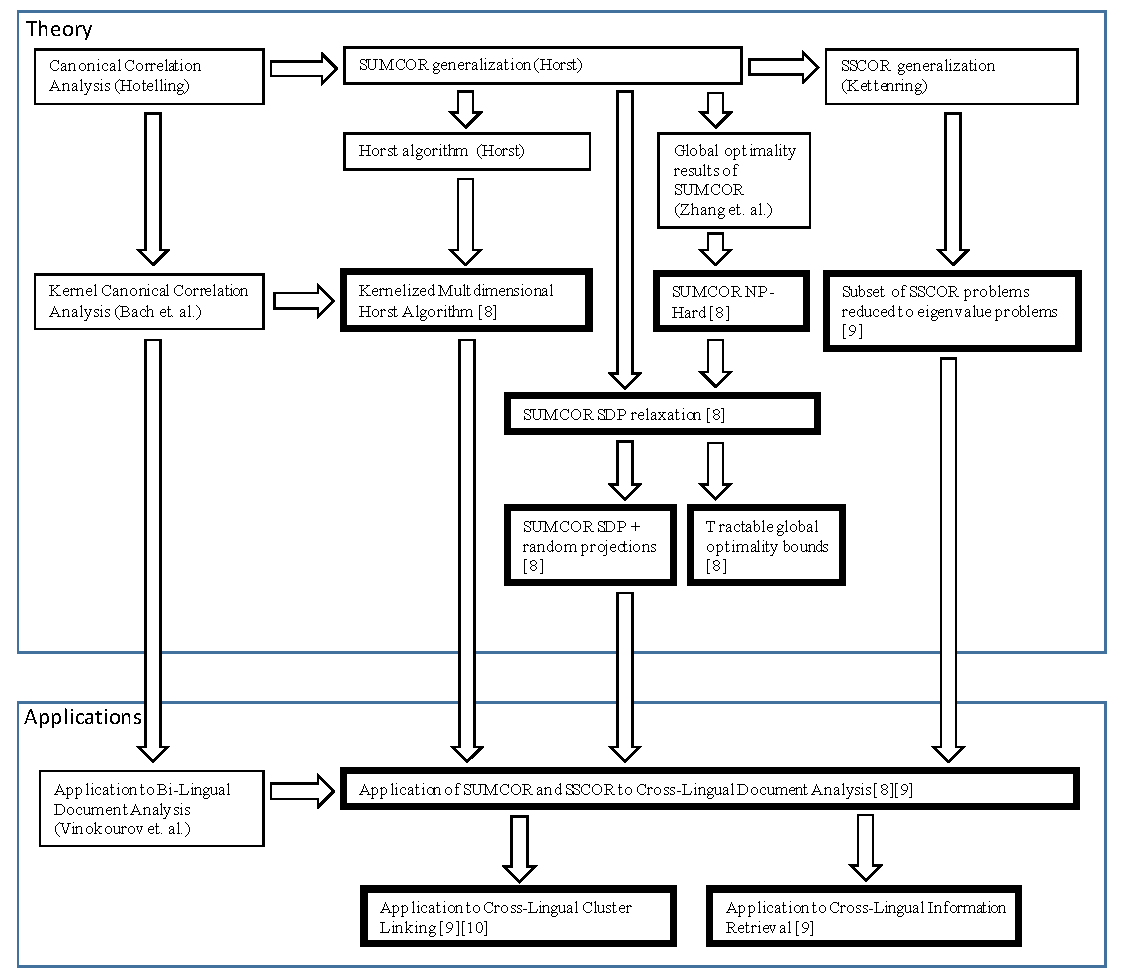
\includegraphics[width=1\textwidth]{figures/position_of_work.pdf}
\caption[The main contributions and related work]{The main contributions, represented by text boxes with thick border, are
positioned with respect to the related work.}
\label{fig:position_of_work}
\end{figure}

\section{Scientific Contributions}

We now list the main scientific contributions of the thesis and their references:
\begin{itemize}
\item A novel algorithm based on the Horst's algorithm that can extract several sets of nonlinear patterns ~\cite{DBLP:journals/corr/abs-1302-0974}
\item A proof that in general the Sum of Correlations problem is NP-hard ~\cite{DBLP:journals/corr/abs-1302-0974}
\item A semidefinite programming relaxation of the SUMCOR problem and
several new bounds on global optimization of the SUMCOR problems~\cite{DBLP:journals/corr/abs-1302-0974}
\item A novel approach to apply the SDP bounds on high-dimensional data~\cite{DBLP:journals/corr/abs-1302-0974}
\item A novel approach to building cross-lingual similarity functions and its application to cross-lingual information retrieval and cross-lingual cluster linking~\cite{rupnikJAIR}\cite{Belyaeva201564}
\item Addressing the missing data problem, a novel reduction of a subset of SSCOR problems to eigenvalue problems~\cite{rupnikJAIR}
\end{itemize}

\section{Thesis Structure}

The rest of the thesis is structured as follows. Chapter~\ref{chap:notation} introduces notation and some
definitions. For background we describe three pattern analysis methods that are the most relevant
for the thesis and explain how they can be adapted for analysis of nonlinear patterns in Chapter~\ref{chap:background}. Chapter~\ref{chap:extensions}
introduces a central problem of the thesis: generalizations of Canonical Correlation Analysis (CCA) and the original
contributions that extend the method to nonlinear and higher-dimensional setting. In Chapter~\ref{chap:relaxations}
we prove the result on the complexity of a particular generalization and study global optimality guarantees based
on semidefinite relaxations. Chapter~\ref{chap:crosslingual} discusses an application of multiview learning
to building cross-lingual similarity models. We show how a particular structure of the data can be exploited
to express a particular generalization of CCA as an eigenvector problem. Chapter~\ref{chap:applications} then
shows how the cross-lingual similarity measures can be used to perform cross-lingual cluster linking, relevant
for large scale monitoring of global news in multiple languages. In Chapter~\ref{chap:experiments} several experiments
are presented both on synthetic and real datasets. Finally, Chapter~\ref{chap:conclusions} concludes the thesis
and discusses possible future directions. 
%
% If needed, the thesis can consist of parts (not encouraged)
%\part{First Part of the Thesis}
%
% Second chapter
%--------------------------------------------------------------------------------------------------
%
\chapter{Background}
%--------------------------------------------------------------------------------------------------

The central subjects in the thesis revolve around statistical approaches to finding structure in one, two or more sets of variates. We will
introduce two methods that find structure in a single set of variates: $k$-means clustering and Principal Component Analysis. We will then present
Canonical Correlation Analysis (CCA), a method for studying two sets of variates. We will also briefly cover kernel method extensions of the methods.


\section{$k$-means}\label{sec:kmeans}

The $k$-means algorithm is perhaps the most well-known and widely-used clustering algorithm. Here, we present its application
to compute cross-lingual similarities. The idea is based on concatenating the corpus matrices, running standard $k$-means clustering to obtain the matrix of centroids, ``reversing" the concatenation step to obtain a set of aligned bases, which are finally used to compute cross-lingual similarities. See Figure~\ref{fig:kmeans} for overview of the procedure. The left side of Figure~\ref{fig:kmeans} illustrates the decomposition and the right side summarizes the coordinate change.

\section{Cross-Lingual Latent Semantic Indexing}\label{sec:LSI}

The second approach we consider is Cross-Lingual Latent Semantic Indexing (CL-LSI)~\cite{cl_lsi} which is a variant of LSI~\cite{lsi} for more than one language. The approach is very similar to $k$-means, where we first concatenate the corpus matrices, compute a decomposition, which in case of CL-LSI is a truncated Singular Value Decomposition (SVD), decouple the
 column space matrix and use the blocks to compute linear maps to a common vector space, where standard cosine similarity is used to compare documents.

 The method is based on computing a truncated singular value decomposition of the concatenated corpus matrix $X \approx U S V^T$. See Figure~\ref{fig:lsi} for the decomposition. Representing documents in ``topic`` coordinates is done in the same way as in the $k$-means case (see Figure~\ref{fig:kmeans}), we will describe how to compute the coordinate change functions.

\begin{figure}[tbp]
\centering
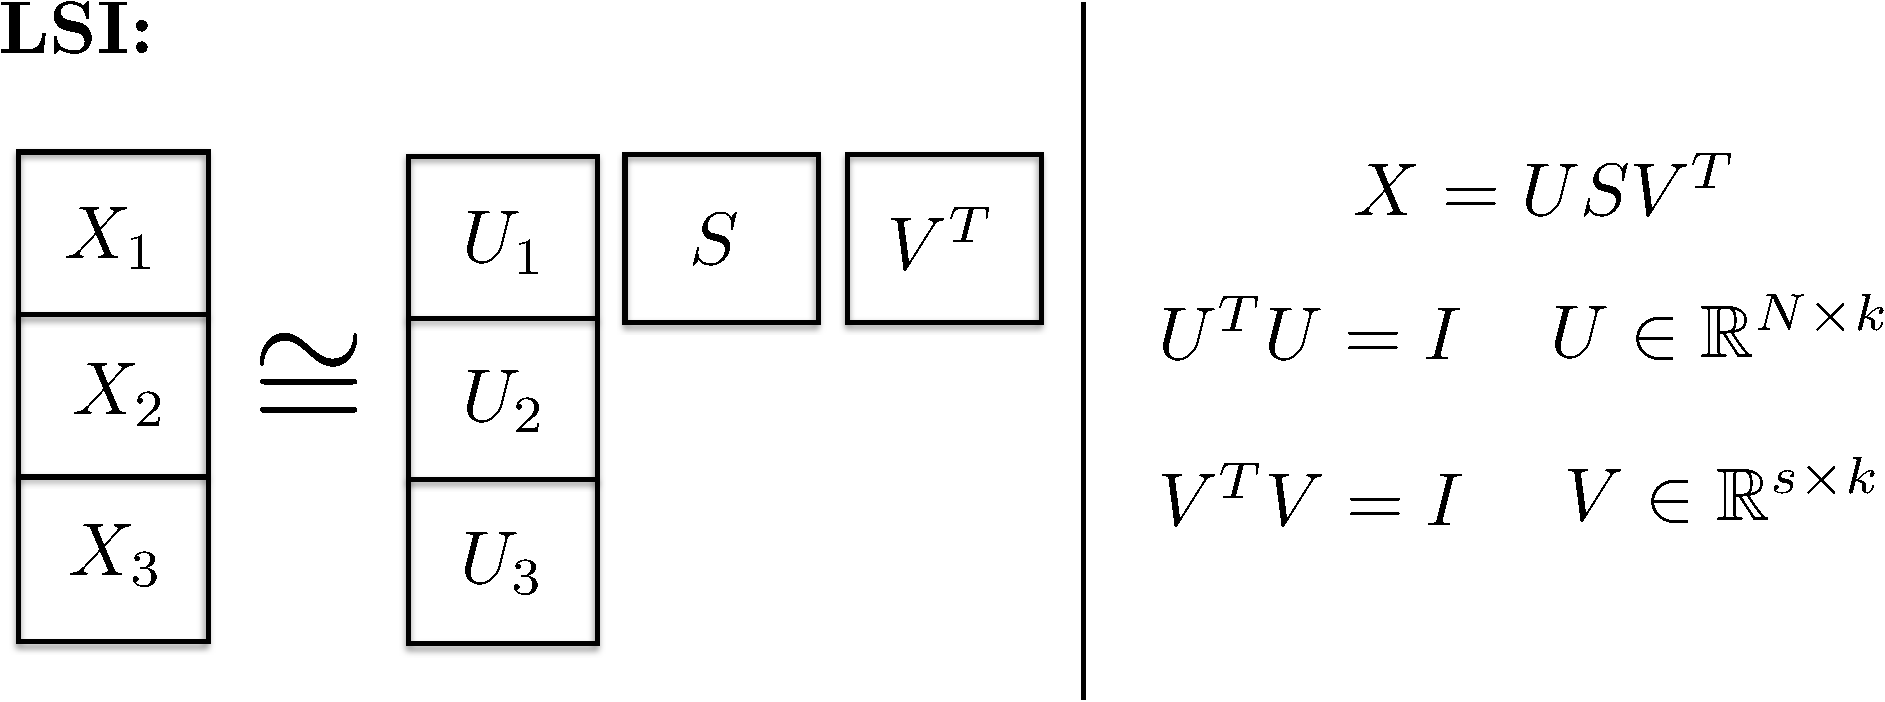
\includegraphics[width=10cm]{figures/lsi.pdf}
\caption{\label{fig:lsi} LSI multilingual corpus matrix decomposition.}
\end{figure}

The cross-lingual similarity functions are based on a rank-$k$ truncated SVD: $X \approx U \Sigma V^T,$ where $U \in \RR^{N \times k}$ are basis vectors of interest and $\Sigma \in \RR^{k \times k}$ is a truncated diagonal matrix of singular eigenvalues. An aligned basis is obtained by first splitting $U$ vertically according to the number of dimensions of each language: $U = [U_1^T \cdots U_m^T]^T$. Then, the same as with $k$-means clustering, we compute the pseudoinverses $P_i = (U_i^T U_i)^{-1} U_i^T$. The matrices $P_i$ are used to change the basis from the standard basis in $\RR^{n_i}$ to the basis spanned by the columns of $U_i$.

\paragraph{Implementation note}

  Since the matrix $X$ can be large we could use an iterative method like the Lanczos algorithm with reorthogonalization~\cite{golub} to find the left singular vectors (columns of $U$) corresponding to the largest singular values. It turns out that the Lanczos method converges slowly as the gap between the leading singular values is small. Moreover, the Lanczos method is hard to parallelize. Instead, we use a randomized version of the SVD~\cite{tropp} that can be viewed as a block Lanczos method. That enables us to use parallelization and speeds up the computation considerably.

To compute the matrices $P_i$ we used the QR algorithm~\cite{golub} to factorize $U_i$ as $U_i = Q_i R_i$, where $Q_i^TQ_i = I$ and $R_i$ is a triangular matrix. $P_i$ is then obtained by solving $R_i P_i = Q_i$.


\section{Canonical Correlation Analysis}

Canonical Correlation Analysis (CCA) ~\cite{Hotelling} is a general procedure for studying relationships between two sets of random variables. It is based on analyzing the cross-covariance matrix between two random vectors with the aim of identifying linear relationships between them. We will start with intuitions and then give a formal presentation.

Roughly speaking, given two random vectors $\mathcal{X}$ and $\mathcal{Y}$ we are interested in "non-trivial" pairs of functions $(f,g)$ such that there is a "dependence" between $f(\mathcal{X})$ and $g(\mathcal{Y})$. The "dependence" we consider is linear (possibly in a Hilbert space). The "non-triviality" of the functions is a requirement that guards us against trivial solutions, such as $f(x) := 0 \cdot x$, $g(y) := 0 \cdot y$ - that is, $f(\mathcal{X})$ and $\mathcal{X}$ should share some information, and analogously for $g(\mathcal{Y})$ and $\mathcal{Y}$. In other words, $f$ and $g$ should not destroy the original signals. When we are interested in more than one good pair of functions, for instance, a family of pairs $(f_i,g_i)$, we typically require additional constraints to prevent non-trivial solutions by enforcing that $f_i\left(\mathcal{X}\right)$ and $f_{j \neq i}\left(\mathcal{X}\right)$ share no information, and similarly for $g_i$. We are interested in essentially different function pairs.

There are several possible applications of such an analysis. For example, a common scenario involves analyzing objects $o \in \mathcal{O}$, where $\mathcal{O}$ is some underlying space, which are not directly observable, but are only observable as images of transformations $F: \mathcal{O} \rightarrow \RR^p$ and $G: \mathcal{O} \rightarrow \RR^q$. That is, we do not have access to $o$ but only to $\left(F(o), G(o)\right)$. Then finding function pairs $(f_i, g_i)$ so that $f_i(F(o))$ behave similarly as $g_i(G(o))$ can be interpreted as finding coupled parametrizations of image spaces of $F$ and $G$ which agree on $\mathcal{O}$. This enables applications such as cross-modal information retrieval, classification, clustering, etc. If $F$ encodes a visual image and $G$ encodes a textual description of the scene, we can perform text input based search over a collection of images, see~\cite{HardoonSS04}. Bi-lingual document analysis is another application, see~\cite{mrpqr}. The pattern functions $(f_i, g_i)$ themselves can be interesting to study for exploratory purposes.

Formally, let
$$ S = \{ \left( F(o_1), G(o_1) \right), \ldots, \left( F(o_n), G(o_n) \right) \} $$
represent a sample of $n$ pairs drawn independently at random according to the underlying distribution, where $F(x_i) \in \RR^p$ and $G(x_i) \in \RR^q$ represent feature vectors from $p$ and $q$-dimensional vector spaces. Let $X=[F(o_1), \ldots, F(o_n)]$ and let $Y=[G(o_1), \ldots ,G(o_n)]$ be the matrices with observation vectors as columns (using MATLAB notation).

The idea is to find two linear functionals (row vectors) $\alpha \in \RR^p$ and $\beta \in \RR^q$ so that the random variables $\alpha \cdot \mathcal{X}$ and $\beta \cdot \mathcal{Y}$ are maximally correlated ($\alpha$ and $\beta$ map the random vectors to random variables, by computing weighted sums of vector components). By using the sample matrix notation $X$ and $Y$ this problem can be formulated as the following optimization problem:

\begin{equation*}
\begin{aligned}
& \underset{\alpha \in \RR^{p}, \beta \in \RR^{q}}{\text{maximize}}
& & \frac{\alpha C_{XY} \beta'}{\sqrt{\alpha C_{XX} \alpha'} \sqrt{\beta C_{YY} \beta'}},
\end{aligned}
\end{equation*}
where $C_{XX}$ and $C_{YY}$ are empirical estimates of variances of $\mathcal{X}$ and $\mathcal{Y}$ respectively and $C_{XY}$ is an estimate for the covariance matrix. Assuming that the observation vectors are centered, the matrices are computed in the following way: $C_{XX} = \frac{1}{n-1}X X'$, $C_{YY} = \frac{1}{n-1}Y Y'$ and $C_{XY} = \frac{1}{n-1}X Y'$.
The optimization problem can be reduced to an eigenvalue problem and includes inverting the variance matrices $C_{XX}$ and $C_{YY}$. If the matrices are not invertible, one can use a regularization technique by replacing $C_{XX}$ with $(1- \kappa)C_{XX} + \kappa I$, where $\kappa \in [0,1]$ is the regularization coefficient and $I$ is the identity matrix.
A single canonical variable is usually inadequate in representing the original random vector and typically one looks for $k$ projection pairs $(\alpha_1, \beta_1),\ldots,(\alpha_k, \beta_k)$, so that $\alpha_i$ and $\beta_i$ are highly correlated and $\alpha_i$ is uncorrelated with $\alpha_j$  for $j \neq i$ and analogously for $\beta$.

The problem can be reformulated as a symmetric eigenvalue problem and solved efficiently. In case the dimensions of the problem $p$ and $q$ are large and observation vectors are sparse, one can consider an iterative method, for example Lanczos algorithm~\cite{LAL}). Alternatively, if the number of observation vectors $n$ is not prohibitively large, one can reformulate the problem to its dual representation which can be combined with a "kernel trick"~\cite{FBMJ} to yield nonlinear version of CCA.

A single canonical variable is usually inadequate in representing the original random vector and typically one looks for $k$ projection pairs $(w_i^1, w_j^1),\ldots,(w_i^k, w_j^k)$, so that $(w_i^{u})^T \mathcal{X}_i$ and $(w_j^{u})^T \mathcal{X}_j$ are highly correlated and $(w_i^{u})^T \mathcal{X}_i$ is uncorrelated with $(w_i^{v})^T \mathcal{X}_i$  for $u \neq v$ and analogously for $w_j^u$ vectors.


\section{Kernels and KCCA}

%
% Third chapter
%--------------------------------------------------------------------------------------------------
%
\chapter{Extensions}
%--------------------------------------------------------------------------------------------------


\section{Introduction}
Natural phenomena are often the product of several factors
interacting. A fundamental challenge of pattern analysis and
machine learning is to find the relationships between these
factors. Real world datasets are often modeled using
distributions such as mixtures of Gaussians.  These models often
capture the uncertainty inherent in both underlying systems and
measurements. Canonical correlation analysis (CCA) is a
well-known and well-developed statistical technique developed to find the
relationships between two sets of random variables.
The relations or patterns discovered by CCA can be used
in two ways. First, they can be used to obtain a common representation for both sets of variables.
Second, the patterns themselves can be used in an exploratory analysis (e.g. see \cite{Hardoon_usingimage}).

It is possible to extend this idea beyond two sets. The
problem is then known as the Multi-set Canonical Correlation Analysis
(MCCA). Whereas it can be shown that CCA can be solved using an
(generalized) eigenvalue computation, MCCA is a much more
difficult problem. One approach is to express it as a
non-convex quadratically constrained quadratic program (QCQP). In
this paper, we show that despite being a highly structured
problem, it is NP-hard. We then describe an efficient algorithm
for finding a locally optimal solutions to the problem.

Since the algorithm is local and the problem non-convex, we
cannot guarantee the quality of the solutions
obtained. Therefore, we give a relaxation of the problem based on
semi-definite programming (SDP) which gives a constant factor
approximation as well as an output sensitive guarantee.

For use in practical applications, we describe two important
extensions: we adapt the methods to use kernels and to find
multi-dimensional solutions.

Finally, we perform extensive experimentation to compare the
efficient local algorithm and the SDP relaxation on both
synthetic and real-world datasets. Here, we show experimentally
that the hardness of the problem is in some sense generic in low
dimensions. That is, a randomly generated problem in low
dimensions will result in many local maxima which are far from
the global optimum. Somewhat surprisingly, this does not occur in
higher dimensions.%, where convergence to solutions that are not globally optimal is rare.

Our contributions in this paper are as follows:
\begin{itemize}
\item We show that in general MCCA is NP-hard.
\item We describe a scalable and efficient algorithm for finding a locally optimal solution.
\item Using an SDP relaxation of the problem, we can compute a
  global upper bound on the objective function along with various
  approximation guarantees on solutions based on this relaxation.
\item We describe two extensions which are important for practical applications: a kernel method and computing multiple sets of canonical vectors.
\item An extensive experimental evaluation of the respective algorithms: we show that in practice the local algorithm performs extremely well, something we can verify with using the SDP relaxation as well as show there are cases where the local algorithm is far from the optimal solution. We do this with a combination of synthetic and real world examples.
\item We propose a preprocessing step based on random projections, which enables us to apply the SDP bounds on large, high dimensional datasets.
\end{itemize}

\vspace{-0.1cm}
\section{Background}\label{sec:Background}
Canonical Correlation Analysis (CCA), introduced by Harold Hotelling \cite{Hotelling},  was developed to detect linear relations between two sets of variables. Typical uses of CCA include
statistical tests of dependence between two random vectors, exploratory analysis on multi-view data, dimensionality reduction and finding a common embedding of two random vectors that share mutual information.

 CCA has been generalized in two directions: extending the method to finding nonlinear relations  by using kernel methods \cite{FBMJ}\cite{HardoonCCA} (see \cite{shawe-taylor04kernel} for an introduction to kernel methods) and extending the method to more than two sets of variables which was introduced in \cite{Kettenring}. Among several proposed generalizations in \cite{Kettenring} the most notable is the sum of correlations (SUMCOR) generalization and it is the focus of our paper. There the goal is to project $m$ sets of random variables to $m$ univariate random variables, which are pair-wise highly correlated on average\footnote{Given $m$ univariate random variables, one can compute $\binom{m}{2}$ correlation coefficients, one for each pair of variables.}. An iterative method to solve the SUMCOR generalization was proposed in \cite{Horst} and the proof of convergence was established in \cite{Chu}. In \cite{Chu} it was shown that a generic SUMCOR problem admits exponentially many locally optimal solutions.
 In \cite{GlobalMEP2} the authors identified a subset of SUMCOR problems for which the iterative procedure converges to a global maximizer (Their results apply to nonnegative irreducible quadratic forms).
In our paper we show that easily computable necessary and sufficient global optimality conditions are theoretically impossible (which follows from the NP-hardness of the problem). Since in
practice good local solutions can be obtained we will present some results on sufficient global optimality.

We also focus on extensions of the local iterative approach \cite{Horst} to make the method practical. Here we show how the method can be extended to finding non-linear patterns and finding more than one set of canonical variates. Our work is related to \cite{JointBSSAppl} where a deflation scheme is used together with the Newton method to find several sets of canonical variates. Our nonlinear generalization is related to \cite{nonlinJointBSS}, where the main difference lies in the fact that we "kernelized" the problem, whereas the authors in \cite{nonlinJointBSS} worked with explicit nonlinear feature representation.

We now list some applications of the SUMCOR formulation. In \cite{kernelHyperAppl} an optimization problem for multi-subject functional magnetic resonance imaging (fMRI) alignment is proposed, which can be formulated as a SUMCOR problem (performing whitening on each set of variables). Another application of the SUMCOR formulation can be found in \cite{JointBSSAppl}, where it is used for group blind source separation on fMRI data from multiple subjects. An optimization problem equivalent to SUMCOR also arises in control theory \cite{ControlApplication} in the form of linear sensitivity analysis of systems of differential equations.
\vspace{-0.1cm}
\section{Sum of Correlations}\label{sec:sumcor}
\paragraph{Notation}
We first introduce the notation we use throughout the paper:
\begin{itemize}
\item Column vectors are denoted by lowercase
letters, e.g. $x$ and matrices are denoted by uppercase letters,
e.g. $X$.
\item Subscripts are used to
enumerate vectors or matrices, e.g. $x_1, x_2$, $X_1$, except in the
special case of the identity matrix, $I_n$ and the zero matrix $0_{k,l}$.
In these cases, the subscripts
denote row and column dimensions.
\item We use MATLAB notation (\cite{golub})% for vector and matrix transpose ($x^T$),
for referring to vector components (e.g. $x(i)$) , matrix elements, rows and columns {(e.g. ${X(i,j), X(i,:), X(:,j)}$)} and vector and matrix concatenation (e.g. $[A B]$).
\item Let $\RR^n$ denote the
$n$-dimensional
real vector space %and $\RR^{n\times m}$ denote
%the $(n \cdot m)$-dimensional vector space used when specifying
%matrix dimensions and let
 %$\NN$ denote the natural numbers and %. Furthermore, let
 and $\sym_n^{+}$ denote the space of symmetric positive definite $n$-by-$n$ matrices.
%\item Let $\norm{v}$ or $\norm{v}_2$ denote the $\ell_2$ norm of the vector $v$ and $\norm{A}_F$, $\norm{A}_1$ and $\norm{A}_2$ to denote the Frobenious norm and 1 and 2 matrix norms.% two commonly used operator norms of matrix $A$.
\end{itemize}
\vspace{-0.1cm}

Before defining  the problem formally, we  give some context and intuition.  Assume we have a random vector $\mathcal{X}$
distributed over $\RR^N$. Without loss of generality, assume it is
centered: $E\left(\mathcal{X}\right) = 0$ and let
$C$ denote the covariance matrix  $Cov\left(\mathcal{X}, \mathcal{X}\right)$. %of $\mathcal{X}$.


\noindent\textbf{Sum of Correlations.}
Canonical Correlation Analysis (CCA) is a method for analyzing two sets of random variables. The goal of CCA is
to identify one-dimensional projections of the two sets of variables that are maximally correlated. We study a generalization with more than two sets of variables.
The key aspect of this problem, which will repeatedly appear, is that we fix number of sets of variables. This assumes that $C$
has a \emph{block structure}. Informally, each block component of $\mathcal{X}$  is a \emph{view} of $\mathcal{X}$, where the views share some mutual information. The problem is to identify the one-dimensional projections of each view that maximize the average correlations across views.
%
%Throughout the paper we will use the block matrix and vector notation.
Let $m$ denote the number of blocks and  $N$ the total number of
elements. Then
$$b := \left(n_1, \ldots, n_m\right), \sum_{i=1}^m b\left(i\right) =
N$$
denotes the number
of elements in each of the blocks. We denote the corresponding
sub-vectors %according to the block structure $b$ are denoted
as $\mathcal{X}^{(i)} \in \RR^{n_i}$
($i$-th block-row of vector $\mathcal{X}$) and the sub-matrices as $C^{(i,j)} \in \RR^{n_i \times n_j}$ ($i$-th block-row, $j$-th block column of matrix $C$); see Figure~\ref{fig:block_structure}. For example, in CCA, there are only two sets, so $m=2$.
\begin{figure}[t]
\centering
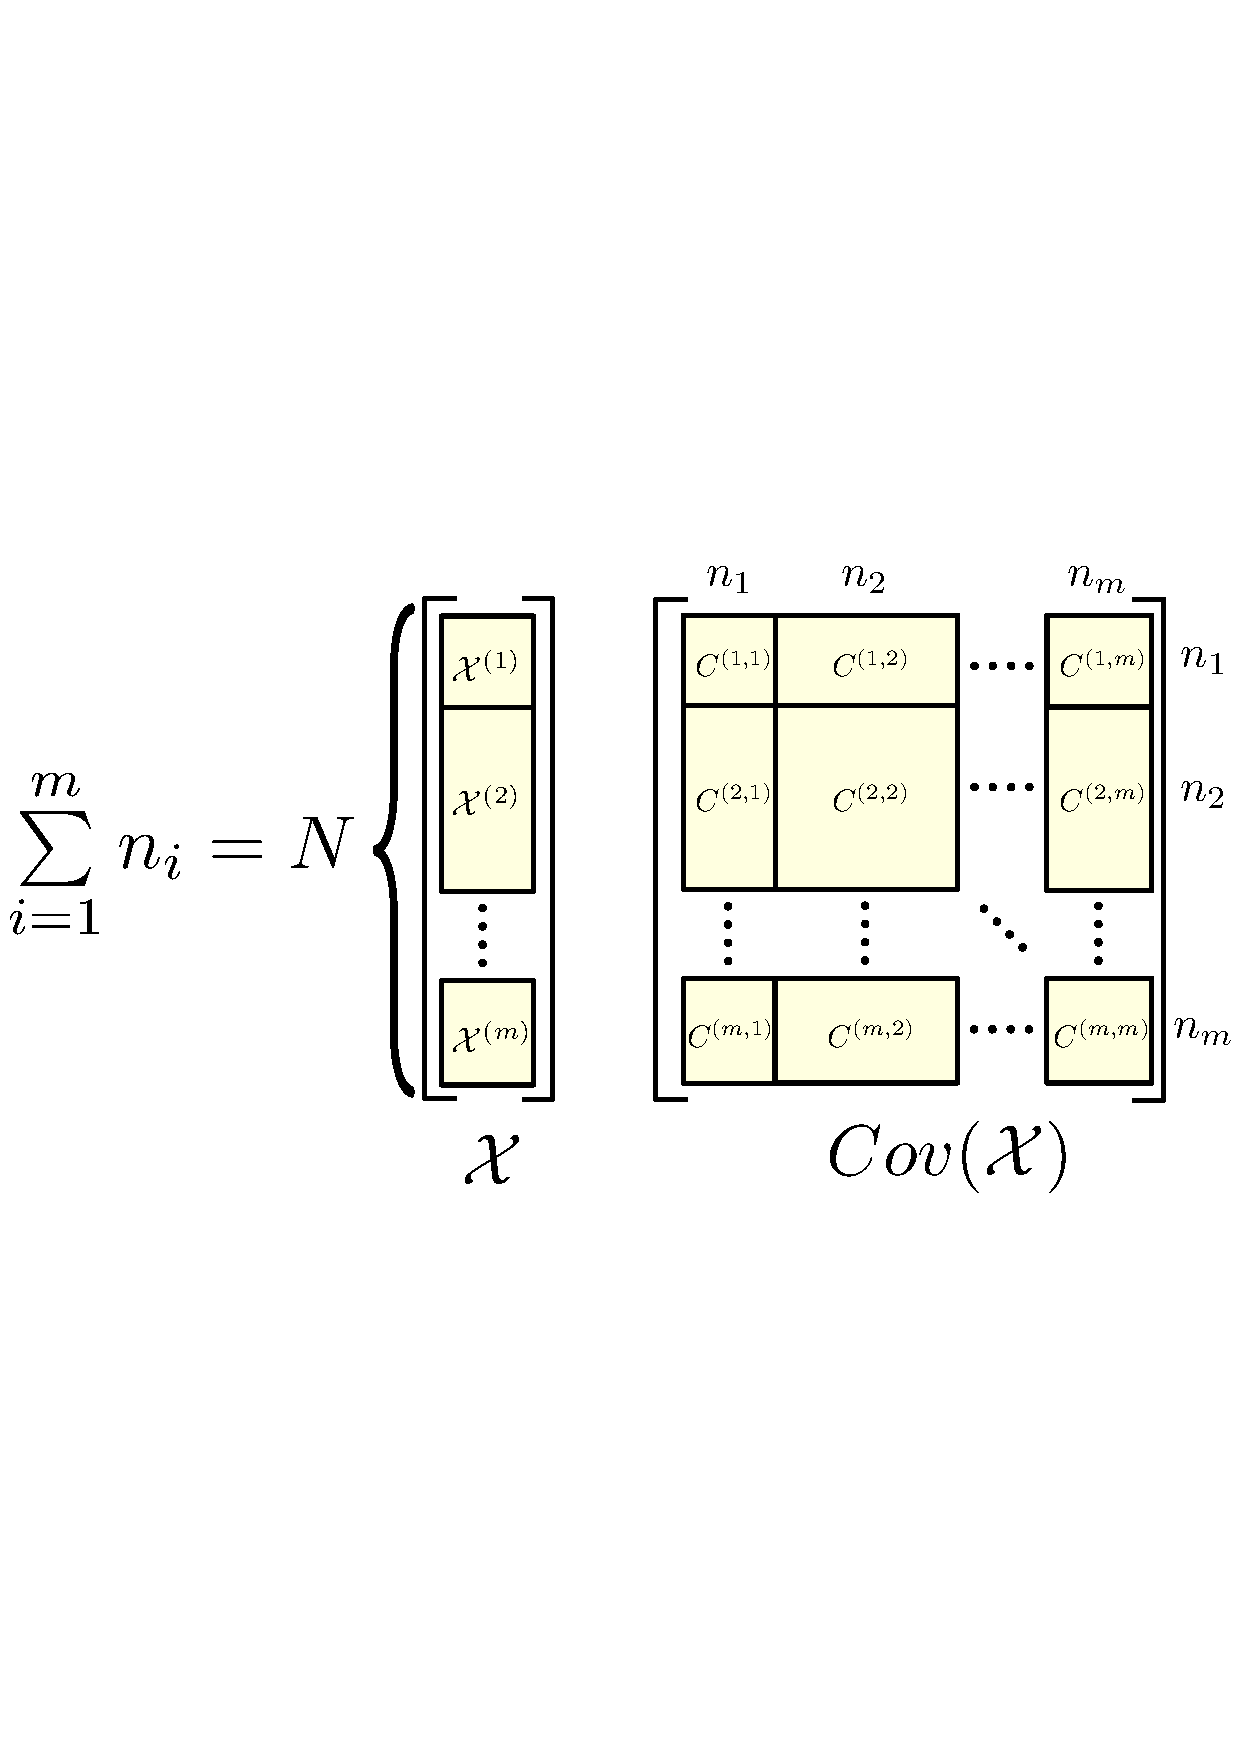
\includegraphics[width=0.5\textwidth]{figures/block_structure.pdf}
\caption{\label{fig:block_structure} The block structure of the  random vector $\mathcal{X}$ and the corresponding covariance block structure.}
\end{figure}
%
%

Formally, given $w \in \RR^N$ we define $m$ random variables $\mathcal{Z}_i$ (one-dimensional projections of random block components of $\mathcal{X}$) as:
\begin{equation*}
\mathcal{Z}_i := \sum_{j = 1}^{n_i} \mathcal{X}^{(i)}\left(j\right)
w^{(i)}\left(j\right) = \mathcal{X}^{(i)T} \cdot w^{(i)}.
\end{equation*}
%$\mathcal{Z}_i$ is a random variable computed as a linear combination of components of $\mathcal{X}^{(i)}$.
%
Let $\rho\left(x,y\right)$ denote the correlation
 coefficient between two random variables:
\begin{equation*}
\rho\left(x,y\right) =
 \frac{Cov\left(x,y\right)}{\sqrt{Cov\left(x,x\right) Cov\left(y,y\right)}}.
\end{equation*}
 The correlation coefficient between $\mathcal{Z}_i$ and
 $\mathcal{Z}_j$ can be expressed as:
\begin{equation*}
\rho\left(\mathcal{Z}_i, \mathcal{Z}_j\right) = \frac{w^{(i)T} C^{(i,j)}
   w^{(j)}}{\sqrt{w^{(i)T} C^{(i,i)} w^{(i)}}\sqrt{w^{(j)T}
     C^{(j,j)} w^{(j)}} }.
\end{equation*}
%
%
The problem described above can be stated as
finding the set of vectors $w^{(i)}$
which maximize
\begin{equation}\label{eq:SUMCOR}
\tag{SUMCOR}
\sum_{i = 1}^m \sum_{j = i+1}^m
\rho\left(\mathcal{Z}_i, \mathcal{Z}_j\right).
\end{equation}
We refer to this problem as Multi-set Canonical
Correlation Analysis (MCCA). Note that it reduces to CCA when
$m=2$. The solution - that is, the set of components $\left(w^{(1)}, \ldots, w^{(m)}\right)$, are referred to as the set of canonical vectors.% We refer to each
%$\mathcal{X}^{(i)}$ as a particular view of some underlying
%object where the assumption is that random vectors
%$\mathcal{X}^{(i)}$ share some mutual information (i.e. are not independent).
%

\noindent\textbf{Reformulating the optimization problem.} Expanding SUMCOR,
we get:
\begin{equation*}
\begin{aligned}
& \underset{w \in \RR^N}{\text{max}} & & \sum_{i = 1}^m
  \sum_{j = i+1}^m \frac{w^{(i)T} C^{(i,j)}
    w^{(j)}}{\sqrt{w^{(i)T} C^{(i,i)} w^{(i)}} \sqrt{w^{(j)T}
      C^{(j,j)} w^{(j)}}}.
\end{aligned}
\end{equation*}
%
%%some explanation
%
Observe that the solution is invariant to scaling (only the direction matters): if $\left(w^{(1)}, \ldots, w^{(m)}\right)$ is a solution, then $\left(\alpha_1 \cdot w^{(1)}, \ldots, \alpha_m \cdot w^{(m)}\right)$ is also a solution for $\alpha_i > 0$. We may therefore impose constraints $w^{(i)T}C^{(i,i)}w^{(i)} = 1$, which only affect the norm. This yields the following
 equivalent constrained problem:
\begin{equation}\label{eq:qcqp0}
\begin{aligned}
& \underset{w \in \RR^N}{\text{maximize}}
& & \sum_{i = 1}^m \sum_{j = i+1}^m w^{(i)T} C^{(i,j)} w^{(j)}\\
& \text{subject to}
& &w^{(i)T} C^{(i,i)} w^{(i)} = 1, \quad\forall i = 1,\ldots, m.
\end{aligned}
\end{equation}
%
We further multiply the objective by $2$ and add a constant $m$. Note that this does not
affect the optimal solution. Using the equalities: $w^{(i)T} C^{(i,j)} w^{(j)} = w^{(j)T} C^{(j,i)} w^{(i)}$ and $w^{(i)T} C^{(i,i)} w^{(i)} = 1$, we obtain:
%
%
\begin{equation}\label{eq:qcqp05}
\begin{aligned}
& \underset{w \in \RR^N}{\text{maximize}}
& & \sum_{i = 1}^m \sum_{j = 1}^m w^{(i)T} C^{(i,j)} w^{(j)}\\
& \text{subject to}
& &w^{(i)T} C^{(i,i)} w^{(i)} = 1, \quad\forall i = 1,\ldots, m.
\end{aligned}
\end{equation}
This transforms the objective function into a quadratic form $w^T C w$. To
simplify the constraints, assume that $C^{(i,i)}$ is strictly positive definite. If $C^{(i,i)}$ is not full rank, then using the eigenvalue decomposition $C^{(i,i)} = V \Lambda V^T$, where $V \in \RR^{n_i \times k}$, $\Lambda \in \RR^{n_i \times k}$, $\Lambda > 0$, $k < n_i$, we substitute $\mathcal{X}^{(i)}$ with $V^T \mathcal{X}^{(i)} \in \RR^k$, for which the covariance matrix is strictly positive definite.
%
%
From the strict positive definiteness it follows that $C^{(i,i)}$ admits a Cholesky decomposition: there exists an invertible matrix $D_i$ such that $C^{(i,i)} = D_i^T D_i$.

Finally, using the block structure $b$, we substitute $w^{(i)}$ with $D_i^{-1} x^{(i)}$ and define $A \in \RR^N$ as:
\begin{equation*}
A^{(i,j)} := {D_i}^{-T} C^{(i,j)} {D_j}^{-1},
\end{equation*}
leading to the simplified problem:
 \begin{equation}\label{eq:qcqp}
\tag{QCQP}
\begin{aligned}
& \underset{x \in \RR^{N}}{\text{max}}
& & x^T A x\\
& \text{subject to}
& &x^{(i)T} x^{(i)} = 1, \quad\forall i = 1, \ldots, m.
\end{aligned}
\end{equation}
It turns out that (\ref{eq:qcqp}) is simpler to  manipulate than  (\ref{eq:SUMCOR}), so we use this form from this point on.





\vspace{-0.1cm}
\section{Extensions}\label{sec:sumcorextensions}
Here we present two extensions of MCCA: how to use kernel methods with
MCCA to find nonlinear dependencies in the data; and an
algorithm to finding more then one set of correlation vectors.
\subsection{Dual representation and kernels}\label{subsec:kernels}
%\label{sect:primal}
We return to formulation (\ref{eq:qcqp0}):
 \begin{equation*}
\begin{aligned}
& \underset{w \in \RR^N}{\text{max}}
& & \sum_{i = 1}^m \sum_{j = i+1 }^m w^{(i)T} C^{(i,j)} w^{(j)}\\
& \text{subject to}
& &w^{(i)T} C^{(i,i)} w^{(i)} = 1, \quad\forall i = 1,\ldots, m,
\end{aligned}
\end{equation*}
  where $b = \left(n_1,\ldots,n_m\right)$ denotes the block structure
  and $ \sum_i n_i = N $.
 In the previous sections, we focused on manipulating covariance matrices only and omitted details on their estimation based on finite samples. In this section, we will use a formulation that explicitly presents the empirical estimates of covariances, which will enable us to apply kernel methods.
Let $\mathcal{X}$ be a random vector distributed over $\RR^N$ with
$E\left(\mathcal{X}\right) = 0$. Let $X \in \RR^{N \times s}$
represent a sample of $s$ observations of $\mathcal{X}$, where each
observation corresponds to a column vector. The empirical covariance of $\mathcal{X}$ based on the sample matrix $X$ is expressed as: $$ \overline{Cov\left(\mathcal{X}\right)} = \frac{1}{s - 1}X X^T.$$
If $s < N$, then $\overline{Cov\left(\mathcal{X}\right)}$ is singular which makes the optimization problem ill-posed and may lead to overfitting (discovering spurious patterns in the data). These issues are addressed by using regularization techniques, typically a shrinkage estimator $\overline{Cov\left(\mathcal{X}\right)_{\kappa}}$ is defined as: $$ \overline{Cov\left(\mathcal{X}\right)_{\kappa}} = \left(1-\kappa\right) \frac{1}{s - 1}X X^T + \kappa  I_N,$$ where $\kappa \in \left[0,1\right]$.

Using the block structure $b$, (\ref{eq:qcqp05}) becomes:
 \begin{equation}\label{eq:regqcqp}
\begin{aligned}
& \underset{w \in \RR^N}{\text{max}}
& & \frac{1}{s -1} \sum_{i = 1}^m \sum_{j = i+1}^m w^{(i)T} X^{(i)}X^{(j)T} w^{(j)} \\
& \text{subject to}
& & w^{(i)T} \left(\frac{1- \kappa}{s - 1}X^{(i)} X^{(i)T} + \kappa  I_N\right) w^{(i)} = 1,\\&&& \quad\forall i = 1,\ldots, m.
\end{aligned}
\end{equation}
To express each component $w^{(i)}$ in terms the columns of $X^{(i)}$,
let $w$ have block structure $b_w = \left(n_1, \ldots, n_m\right)$
where $\sum_i n_i = N$, and let $y \in \RR^{m\cdot s}$ have block
structure $b_y\left(i\right) = s, \forall i = 1,\ldots, m$. The
component $w^{(i)}$ can be expressed as:
\begin{equation}\label{eq:representer}
\begin{aligned}
w^{(i)} = \sum_{j = 1}^{s} y^{(i)}\left(j\right) X^{(i)}\left(:,j\right) = X^{(i)} y^{(i)}.
\end{aligned}
\end{equation}
We refer to $y$ as dual variables.
%
%
%It remains to check that the formulations (\ref{eq:regqcqp}) and (\ref{eq:dualregqcqp}) are equivalent. We need to check that the optimal solution to (\ref{eq:regqcqp}) can be expressed by using dual variables \eqref{eq:representer}.
\begin{lemma}
There exists a solution to \eqref{eq:regqcqp} which can be expressed as \eqref{eq:representer}.
\end{lemma}
\begin{proof}
We prove the lemma by contradiction. Assume that no optimal solution
can be expressed as \eqref{eq:representer} and $u$ be an optimal solution to the problem \eqref{eq:regqcqp}. Without loss of generality, assume that $u^{(1)}$ does not lie in the column space of $X^{(1)}$:
 $$u^{(1)} = z_{\bot} + X^{(1)} y^{(1)},$$
 where
$$z_{\bot} \neq 0_{n_1}\quad \text{and}\quad X^{(1)T}z_{\bot} = 0_s.$$
We show that $\bar{u}$, defined as $\bar{u}^{(i)} := u^{(i)}, \forall i> 1$ and $\bar{u}^{(1)} := \frac{1}{\gamma}  X^{(1)} y^{(1)},$ where
\begin{equation*}
\gamma :=\sqrt{ y^{(1)T} X^{(1)T} \left(\frac{1- \kappa}{s - 1}X^{(1)} X^{(1)T} + \kappa  I_N\right) X^{(1)} y^{(1)} },
\end{equation*}
strictly increases the objective function, which contradicts the assumption that $u$ is optimal. Clearly, $\bar{u}$ is a feasible solution. Positive definiteness of $\frac{1- \kappa}{s - 1}X^{(1)} X^{(1)T} + \kappa  I_N$, coupled with the fact that $z_{\bot}^T z_{\bot} > 0$ implies that $0 < \gamma < 1$. Let $E := \sum_{j = 2}^m \left(X^{(1)} y^{(1)}\right)^T X^{(1)}X^{(j)T} u^{(j)}$.
%
If $E < 0$, then the
vector $[-u^{(1)T} u^{(2)T} \cdots u^{(m)T}]^T$ strictly increases the
objective function, which is a contradiction. We also obtain a contradiction if $E = 0$, since any nonzero $v \in \RR^{s}$ for which $X^{(1)}v \neq 0_{n_1}$ can be used to obtain a solution to the problem \eqref{eq:regqcqp} expressed as \eqref{eq:representer} (after re-scaling  such that $\overline{Cov\left(\mathcal{X}^{(1)}v\right)_\kappa} = 1$ and if necessary multiplying it by $-1$ so that $\sum_{j = 2}^m \left(X^{(1)} v\right)^T X^{(1)}X^{(j)T} u^{(j)}) \geq 0$).
Thus, we may assume that $E > 0$.
%If the sum was zero, then any properly scaled (with proper sign) combination of the training data $X^{(1)}$ could be used in place of $u^{(1)}$).
%
The following inequality completes the proof, since it shows that $\bar{u}$ increases the objective function:
%Note that $\frac{1}{s -1}  u^{(i)T} X^{(i)}X^{(j)T} u^{(j)} = \frac{1}{s -1}  \bar{u}^{(i)T} X^{(i)}X^{(j)T} \bar{u}^{(j)}$ where $i > 1$ and $j > 1$ and $u^{(1)T} (\frac{1- \kappa}{s - 1}X^{(1)} X^{(1)T} + \kappa  I_N) u^{(1)} = \bar{u}^{(1)T} (\frac{1- \kappa}{s - 1}X^{(1)} X^{(1)T} + \kappa  I_N) \bar{u}^{(1)} = 1$.
\begin{align*}
  \frac{1}{s -1} & \sum_{j = 2}^m u^{(1)T} X^{(1)}X^{(j)T} u^{(j)} =\\
= \frac{1}{s -1} & \sum_{j = 2}^m \left(z_{\bot} + X^{(1)} y^{(1)}\right)^T X^{(1)}X^{(j)T} u^{(j)} = \\
= \frac{1}{s -1}  &\sum_{j = 2}^m \left(X^{(1)} y^{(1)}\right)^T X^{(1)}X^{(j)T} u^{(j)} < \\
< \frac{1}{s -1}  &\sum_{j = 2}^m \frac{1}{\gamma}\left(X^{(1)} y^{(1)}\right)^T X^{(1)}X^{(j)T} u^{(j)}.
\end{align*}
%\qed
\end{proof}


%\substack{j = 1\\ j\neq i}

Let $K_i = X^{(i)T} X^{(i)} \in \RR^{s \times s}$ denote the Gram
matrix. Next, we express the problem (\ref{eq:regqcqp}) in terms of the dual variables:
 \begin{equation}\label{eq:dualregqcqp}
\begin{aligned}
& \underset{y \in \RR^{m\cdot s}}{\text{max}}
& & \frac{1}{s -1} \sum_{i = 1}^m \sum_{j = i+1}^m y^{(i)T} K_i K_j^T y^{(j)} \\% + \sum_{i = 1}^m y^{(i)T} (\frac{1 - \kappa}{s - 1}K_i  K_i^T + \kappa  K_i) y^{(i)}\\
& \text{subject to}
& & y^{(i)T} \left(\frac{1- \kappa}{s - 1}K_i K_i^T + \kappa  K_i\right) y^{(i)} = 1,\\
& &&\quad\forall i = 1,\ldots, m.
\end{aligned}
\end{equation}
Expressing the problem in terms of Gram matrices makes it amenable to using kernel methods (see \cite{shawe-taylor04kernel}).% which
%enable discovering nonlinear patterns in the data.


Typically the matrices $K_i$ are ill conditioned (or even singular
when the data is centered) and it is advantageous to constrain the
magnitude of dual coefficients as well as the variance in the original
problem. We address this by introducing a first order approximation to
the dual regularized variance.  Let $$\widetilde{K_i} :=
\left(\sqrt{\frac{1-\kappa}{s - 1}}K_i + \frac{\kappa}{2}
  \sqrt{\frac{s-1}{1- \kappa}}I_s\right).$$ The covariance becomes:
%
 $$ \overline{Cov\left(\mathcal{X}^{(i)}\right)_{\kappa}} =  \frac{1- \kappa}{s - 1}K_i K_i^T + \kappa  K_i \approx  \widetilde{K_i} \widetilde{K_i}^T.$$
This approximation has two advantages: it is invertible and is in a
factorized form. We exploit the latter when obtaining a convergent local method.
The final optimization is then expressed as:
 \begin{equation}\label{eq:approxdualqcqp}
\begin{aligned}
& \underset{y \in \RR^{m\cdot s}}{\text{max}}
& & \frac{1}{s -1} \sum_{i = 1}^m \sum_{j = i+1}^m y^{(i)T} K_i K_j^T y^{(j)}\\% + \sum_{i = 1}^m y^{(i)T} \widetilde{K_i} \widetilde{K_i}^T y^{(i)}\\
& \text{subject to}
& & y^{(i)T} \widetilde{K_i} \widetilde{K_i}^T y^{(i)} = 1, \quad\forall i = 1,\ldots, m.
\end{aligned}
\end{equation}
%
The problem can be interpreted as maximizing covariance while constraining variance and magnitude of dual coefficients. %Notice that the sum in the objective $\sum_{i = 1}^m y^{(i)T} \widetilde{K_i} \widetilde{K_i}^T y^{(i)}$ is constant and thus redundant. It is useful to keep it in order to obtain a reformulation of the problem where the local method provably converges.

%\subsection{Regularization}
%To prevent overfitting and make the problem numerically stable (as in CCA) we propose a regularization scheme. Let $\kappa \in [0,1]$ and let $\tilde{K}_i := (1-\kappa)K_i + \kappa I$, solve:
%\begin{equation}\label{equation:regdual}\max_{\beta_1, \ldots, \beta_m} \sum_{i < j} \beta_i' K_i K_j \beta_j,\end{equation} s.t. $$\beta_i'\tilde{K}_i \tilde{K}_i \beta_i = 1, \quad \forall i.$$
%The main benefit of this form of regularization is the a priori Cholesky-like decomposition (the factors are not triangular). This form of regularization is provably equivalent to regularization in \cite{FBMJ}.


\subsection{Computing several sets of canonical vectors}\label{subsec:severalCanonicalVectors}
Usually a one-dimensional representation does not sufficiently capture
all the information in the data and higher dimensional subspaces are
needed. After computing the first set of primal canonical vectors we
proceed to computing the next set. The next set should be almost as
highly correlated as the first one, but essentially ``different'' from
the first one. We achieve this by imposing additional constraints for
every view. Namely, all projection vectors in view $i$ are
uncorrelated with respect to $\widetilde{K}_i^2$ (this is similar to
the approach in two view regularized kernel CCA\cite{FBMJ}).
\par
Let $Y = \left[y_1, \ldots, y_k\right] \in \RR^{m\cdot s  \times k}$ represent $k$ sets of canonical vectors, where
$$Y^{(\ell)T} \widetilde{K_{\ell}^2} Y^{(\ell)} = I_k  \quad\forall \ell = 1,\ldots, m. $$
The equation above states that each canonical vector has unit regularized variance and that different canonical vectors corresponding to the same view are uncorrelated (orthogonal with respect to $\widetilde{K_i^2}$).


%%\delta_{ij} \forall \ell = 1,\ldots, m$$
%%where $$\delta_{ij}  = \left\{ \begin{array}{lll}
%%0 & {\rm for} ~i \neq j \\
%%1 & {\rm for} ~i = j   \end{array} \right.$$

%%_i = (y_i^1, \ldots, y_i^k)$ is the matrix
%%of $k$ uncorrelated vectors with respect to $\tilde{K}_i$, for every
%%view $i$. We are searching for the set of vectors $\beta_1^{k+1},
%%\ldots, \beta_m^{k+1}$ with unit regularized variance that maximize
%%the \textsc{sumcor} objective and are uncorrelated with the first $k$
%%solutions:
%%$${\beta_i^{k+1}}' \tilde{K}_i^2 \beta_i^{j}, \forall j < k+1, \forall i,$$
%%which can be written as:
%%$${\beta_i^{k+1}}'\tilde{K}_i^2 B_i = 0 , \forall i.$$

We will now extend the set of constraints in the optimization (\ref{eq:approxdualqcqp}) to enforce the orthogonality.
%
 \begin{equation}\label{eq:kdimapproxdualqcqp}
\begin{aligned}
& \underset{y \in \RR^{m\cdot s}}{\text{max}}
& & \frac{1}{s -1} \sum_{i = 1}^m \sum_{j = i+1}^m y^{(i)T} K_i K_j^T y^{(j)}\\% + \sum_{i = 1}^m y^{(i)T} \widetilde{K_i} \widetilde{K_i}^T y^{(i)}\\
& \text{subject to}
& & y^{(i)T} \widetilde{K_i} \widetilde{K_i}^T y^{(i)} = 1, \quad\forall i = 1,\ldots, m\\
& & & Y^{(i)T} \widetilde{K_i} \widetilde{K_i}^T y^{(i)} = 0_k, \quad\forall i = 1,\ldots, m.
\end{aligned}
\end{equation}
%
%
To use the Horst algorithm, we first use the substitutions:
$$Z^{(i)} = \widetilde{K_i}Y^{(i)}, \quad z^{(i)} = \widetilde{K_i}y^{(i)}$$
and define the operators $$P_i = I_s - \widetilde{K}_i Y^{(i)} Y^{(i)T} \widetilde{K}_i = I_s - Z^{(i)} Z^{(i)T},$$ which map to the space orthogonal to the columns of $\widetilde{K}_i Y^{(i)}$. Each $P_i$ is a projection operator: $P_i^2 = P_i,$ which follows directly from the identities above.
The optimization problem in the new variables is:
%
 \begin{equation}\label{eq:Zkdimapproxdualqcqp}
\begin{aligned}
& \underset{z \in \RR^{m\cdot s}}{\text{max}}
& & \frac{1}{s -1} \sum_{i = 1}^m \sum_{j = i+1}^m z^{(i)T} \widetilde{K_i}^{-T} K_i K_j^T \widetilde{K_j}^{-1} z^{(j)} \\%+ \sum_{i = 1}^m z^{(i)T} z^{(i)}\\
& \text{subject to}
& & z^{(i)T}  z^{(i)} = 1, \quad\forall i = 1,\ldots, m\\
& & & Z^{(i)T} z^{(i)} = 0_k, \quad\forall i = 1,\ldots, m.
\end{aligned}
\end{equation}
%
%
%
Using the projection operators, this is equivalent to:
\begin{equation*}%\label{eq:projZkdimapproxdualqcqp}
\begin{aligned}
& \underset{z \in \RR^{m\cdot s}}{\text{max}}
& & \frac{1}{s -1} \sum_{i = 1}^m \sum_{j = i+1}^m z^{(i)T} P_i^T \widetilde{K_i}^{-T} K_i K_j^T \widetilde{K_j}^{-1} P_j z^{(j)}\\% + \sum_{i = 1}^m z^{(i)T}  z^{(i)}\\
& \text{s.t.}
& & z^{(i)T}  z^{(i)} = 1, \quad\forall i = 1,\ldots, m.
\end{aligned}
\end{equation*}
%
By multiplying the objective by $2$ (due to the symmetries of $P_i, K_i$ and $\widetilde{K_i}$) and shifting the objective function by $\frac{m}{1 - \kappa}$, the problem is equivalent to:
\begin{equation}%\label{eq:projZkdimapproxdualqcqp}
\begin{aligned}
& \underset{z \in \RR^{m\cdot s}}{\text{max}}
& & \frac{1}{s -1} \sum_{i = 1}^m \sum_{\substack{j = 1\\ j\neq i}}^m z^{(i)T} P_i^T \widetilde{K_i}^{-T} K_i K_j^T \widetilde{K_j}^{-1} P_j z^{(j)}\\
&&& + \frac{1}{1-\kappa}\sum_{i = 1}^m z^{(i)T}  z^{(i)}\\
& \text{s.t.}
& & z^{(i)T}  z^{(i)} = 1, \quad\forall i = 1,\ldots, m.
\end{aligned}
\end{equation}
%
%
%
This optimization can be reformulated as:
\begin{equation}\label{eq:projZkdimapproxdualqcqp}
\begin{aligned}
& \underset{z \in \RR^{m\cdot s}}{\text{max}}
& & z^T A z\\
& \text{subject to}
& & z^{(i)T}  z^{(i)} = 1, \quad\forall i = 1,\ldots, m,
\end{aligned}
\end{equation}
where $A \in \RR^{m\cdot s}$ with block structure $b\left(i\right) = s, \forall i = 1,\ldots, m$, defined by:
\begin{equation*}
 A^{(i,j)} = \left\{ \begin{array}{lll}
 \frac{1}{s -1} P_i^T \widetilde{K_i}^{-T} K_i K_j^T \widetilde{K_j}^{-1} P_j  & {\rm for} ~i \neq j\\
\frac{1}{1-\kappa } I_s & {\rm for} ~i = j \end{array}\right\}.
\end{equation*}
%
\begin{lemma}
The block matrix $A$ defined above is positive semidefinite (i.e. $A \in \sym_+^{m\cdot s}$).
\end{lemma}
\begin{proof}
$A$ is symmetric, which follows from $P_i = P_i^T$ and $K_i =
K_i^T$. Let $z \in \RR^{m\cdot s}$.  The goal is to show that $z^T A z > 0$.
Let us define an auxiliary matrix $W$ as:
\begin{equation*}
\begin{aligned}
W =  \frac{1}{1- \kappa }&\sum_{i = 1}^m z^{(i)T} P_i^T
\widetilde{K_i}^{-T} \cdot \\&\left( \kappa K_i + \frac{\kappa^2
    \left(s-1\right)}{4\left(1-\kappa\right)}I_s   \right)
\widetilde{K_i}^{-1} P_i z^{(i)}
\end{aligned}
\end{equation*}
 Each summand is positive-semidefinite, i.e. $W \geq 0$ and $W > 0$ if $\exists i: P_i z^{(i)} = z^{(i)}$. What follows is a sequence of inequalities, some of which must
 be strict, as will be established:
\begin{align}
z^T A z &=  \frac{1}{s -1} \sum_{i = 1}^m \sum_{\substack{j = 1\\j\neq i}}^m z^{(i)T} P_i^T \widetilde{K_i}^{-T} K_i K_j^T \widetilde{K_j}^{-1} P_j z^{(j)}\nonumber
\\& \qquad + \frac{1}{1- \kappa }\sum_{i = 1}^m z^{(i)T}  z^{(i)} \label{proof_line_1}\\
%
&\geq \frac{1}{s -1} \sum_{i = 1}^m \sum_{\substack{j = 1\\ j\neq i}}^m z^{(i)T} P_i^T \widetilde{K_i}^{-T} K_i K_j^T \widetilde{K_j}^{-1} P_j z^{(j)}\nonumber\\
& \qquad + \frac{1}{1- \kappa }\sum_{i = 1}^m z^{(i)T} P_i^T P_i z^{(i)}  \label{proof_line_2}\\
%
 &= \frac{1}{s -1} \sum_{i = 1}^m \sum_{\substack{j = 1\\ j\neq i}}^m z^{(i)T} P_i^T \widetilde{K_i}^{-T} K_i K_j^T \widetilde{K_j}^{-1} P_j z^{(j)}\nonumber\\
 & \qquad+ \frac{1}{1- \kappa }\sum_{i = 1}^m z^{(i)T} P_i^T \widetilde{K_i}^{-T}  \widetilde{K_i}^T \widetilde{K_i} \widetilde{K_i}^{-1} P_i z^{(i)}  \label{proof_line_3}\\
%
&= \frac{1}{s -1} \sum_{i = 1}^m \sum_{\substack{j = 1\\ j\neq i}}^m z^{(i)T} P_i^T \widetilde{K_i}^{-T} K_i K_j^T \widetilde{K_j}^{-1} P_j z^{(j)}\nonumber
\\& \qquad+ \frac{1}{s-1}\sum_{i = 1}^m z^{(i)T} P_i^T \widetilde{K_i}^{-T}  K_i K_i^T \widetilde{K_i}^{-1} P_i z^{(i)} + W  \label{proof_line_4}\\
%+ \frac{1}{1- \kappa }&\sum_{i = 1}^m z^{(i)T} P_i^T \widetilde{K_i}^{-T} \left( \kappa K_i + \frac{\kappa^2 \left(s-1\right)}{4\left(1-\kappa\right)}I_s   \right) \widetilde{K_i}^{-1} P_i z^{(i)}
 &= z^T B B^T z + W \geq 0\nonumber,
\end{align}
where $B \in \RR^{m\cdot s \times s}$, defined by $B^{(i)} = \frac{1}{\sqrt{s-1}}(K_i \widetilde{K_i}^{-1}P_i)^T$, with corresponding row block structure $b\left(i\right) = s$. The inequality after (\ref{proof_line_1}) holds since projection operators cannot increase norms.
(\ref{proof_line_3}) is equal to (\ref{proof_line_2}) using $\widetilde{K_i}^{-T}  \widetilde{K_i}^T = I$.
Regrouping the terms and applying the definition of $W$, we obtain (\ref{proof_line_4}).
The final equality follows, since the first two sums form a perfect square.

Now we will show that at least one of the two inequalities is strict. If $P_i z^{(i)} \neq z^{(i)}$ for some $i$, then the first inequality is strict ($\norm{P_i z^{(i)}} < \norm{z^{(i)}}$). Conversely, if $P_i z^{(i)} = z^{(i)}$ for all $i$, then $W > 0$, hence the last inequality is strict.%\qed
\end{proof}



Matrix $A$ has all the required properties for convergence, so we
apply Algorithm \ref{algorithm:horst}. Solutions to
\eqref{eq:kdimapproxdualqcqp} are obtained by back-substituting into $y^{(i)} = \widetilde{K_i}^{-1} z^{(i)}$.


%%\begin{equation}\max_{y \in \RR^{m\cdot s}} \sum_{i < j} \beta_i' K_i K_j \beta_j   + \frac{1}{2(1-\kappa)^2}\sum_i \beta_i' \tilde{K}_i^2 \beta_i,\end{equation} s.t. $$\beta_i'\tilde{K}_i \tilde{K}_i \beta_i = 1, \quad \forall i$$\begin{equation}{B_i^k}' \tilde{K}_i^2 \beta_i = 0, \forall i.\end{equation}
%
%The solution to the above problem can be found by solving the following MEP:
%
%$$\sum_{j \neq i}P_i \tilde{K}_i^{-1} K_i K_j\tilde{K}_j^{-1} P_j
%\alpha_j + \frac{1}{(1-\kappa)^2}\alpha_i +  \lambda_i \alpha_i = 0,
%\forall i.$$
%
%followed by multiplying the solutions $\alpha_i$ by $\tilde{K}_i^{-1}$.
%
%Eigenvalue shifting techniques can be applied to force positive-definiteness (details omitted).
% The algorithm is
%shown in Algorithm \ref{fullalg}.
%

%\begin{algorithm}
%\caption{Horst algorithm for computing a $k$-dimensional representation}
%Input: $K_1, \ldots, K_m$, $\kappa$, $maxiter$, $k$, \par
%Output: $B_1^k, \ldots, B_m^k$
%\begin{algorithmic}
%\label{fullalg}
%\STATE $\tilde{K}_i = (1-\kappa) K_i +  \kappa I, \forall i$
%\FOR{$d = 1$ to $k$}
%\STATE Choose random vectors $\alpha_1^0, \ldots, \alpha_m^0$
%\IF{$d > 1$}
%\STATE $P_i^d =I -  \tilde{K}_i B_i^{d-1} {B_i^{d-1}}' \tilde{K}_i$
%\STATE Set $\alpha_i^0 \leftarrow P_i^d \alpha_i^0,~~~~ \forall i$
%\ELSE
%\STATE  $P_i^d = I ~~~~ \forall i$
%\ENDIF
%\STATE $u_i^0 = K_i \tilde{K}_i^{-1} \alpha_i^0, \forall i$
%\FOR{$i = 1$ to $maxiter$}
%\FOR{$j =1$ to $m$}
%\STATE $\alpha_j^{i} \leftarrow  P_j^d \tilde{K}_j^{-1} K_j \sum_{k\neq j}  u_k^{i-1}  + \left(\frac{1}{(1-\kappa)^2} \right) \alpha_j^{i-1}$
%\STATE $\alpha_j^{i} \leftarrow \frac{\alpha_j^{i}}{\sqrt{{\alpha_j^i}' \alpha_j^i}}$
%\STATE $u_j^{i} \leftarrow  K_k  \tilde{K}_k^{-1}  \alpha_k^{i}$
%\ENDFOR
%\ENDFOR
%\FOR{$l = 1$ to $m$}
%\STATE $\beta_l^d = \tilde{K}_l^{-1} \alpha_l^{maxiter}$
%\STATE $B_l^{d} = [ B_l^d , \beta_l^d]$ if $d > 1$
%\STATE $B_l^{d} = [ \beta_l^d]$ if $d = 1$
%\ENDFOR
%\ENDFOR
%\end{algorithmic}
%\end{algorithm}



\subsection{Implementation}\label{subsec:implementation}
The algorithm requires matrix vector multiplications and inverted
matrix vector multiplications. If the kernel matrices are products of
sparse matrices: $K_i = X^{(i)T} X^{(i)}$ with each $X^{(i)}$ having
$s\cdot n$ elements
where $s << n$, then the kernel matrix vector multiplications cost is $2 n s$
rather than $n^2$. Rather than computing the full inverses, we solve
the system $K_i x = y$ for $x$, every time $K_i^{-1} y$ is needed. Since
regularized kernels are symmetric and multiplying them with vectors is
fast (roughly four times slower than multiplication with the original sparse matrices $X^{(i)}$), an iterative method like conjugate gradient (CG) is
suitable. Higher regularization parameters increase the condition
number of each $\tilde{K}_i$ which speeds up CG convergence.
\par
If we fix the number of iterations, $maxiter$, and number
of CG steps, $C$, the computational cost of computing a
$k$-dimensional representation is upper bounded by: $O\big(C \cdot
maxiter \cdot k^2 \cdot m \cdot n \cdot s \big),$ where $m$ is the
number of views, $n$ the number of observations and $s$ average number
of nonzero features of each observation.
%
Since the majority of computations are  sparse matrix-vector multiplications, the
algorithm can be parallelized (the sparse matrices are fixed and can be split into multiple
blocks).

So far, we have assumed that the data is centered. Centering can efficiently be implemented on the
fly with no changes in asymptotic computational complexity, but we omit the technical details due to space constraints.

\section{Discussion}\label{sec:discussion}

In the paper we studied a generalization of CCA to more than two
sets of variables. We showed that the complexity of the problem
is NP-hard and described a locally convergent method as well as
presented how to generalize the method to the nonlinear case with
several canonical variates.  Experimentally, we observe that the
performance of the local method (with linear convergence) is
generally good, although we identified problem settings where the
local method can be far from globally optimal. We presented a
SDP relaxation of the problem, which can be used to obtain new
local solutions and to provide certificates of optimality. The
usefulness of the bounds was tested on synthetic problem
instances and a problems related to cross-lingual text
mining. We introduced a new preprocessing step based on random
projections to reduce the dimensionality of high dimensional problems
such as in document corpora, making memory requirements tractable.
% The high dimensional nature of documents and the size of
% the document collections result in untractable memory
% requirements. We solved the issue by proposing a preprocessing
% step based on random projections.
Future work includes analyzing the complexity of the other
generalizations proposed in \cite{Kettenring}. We found that
noisy 1-dimensional embeddings present difficulties for the local
approach as opposed to generic problem structures. A natural
question is, are there other problem structures that result in
suboptimal behavior of the local approach? Our empirical results were
based text data, but we plan to extend this analysis to data from other modalities, such as images, sensor streams and graphs.
%
%\part{Second Part of the Thesis}
%
% Fourth chapter
%--------------------------------------------------------------------------------------------------
% 
\chapter{Definitions and Theorems}
%--------------------------------------------------------------------------------------------------

\section{Definitions}

See the formal definition of the right triangle in Definition~\ref{def:right-triangle}.

\begin{definition}[Right triangle]
\label{def:right-triangle}
A \emph{right triangle} is a triangle in which one angle is a 90-degree angle.
\end{definition}

\section{Theorems}
\label{sec:theorems}

The Pythagorean theorem is a relation in Euclidean geometry among the three sides of a right triangle. It states that the square of the hypotenuse (the side opposite the right angle) is equal to the sum of the squares of the other two sides \parencite{pythagoras}. \index{Pythagorean theorem!theorem}

\begin{theorem}[Pythagorean theorem]
\label{thm:pythagoras}
In every right triangle with sides $a$ and $b$ and hypotenuse $c$, the following holds:
\begin{equation}
a^2 + b^2 = c^2
\end{equation}
\end{theorem}

See Appendix~\ref{app:proofs} for the proof of this theorem.
%
% Fifth chapter
%--------------------------------------------------------------------------------------------------
%
\chapter{Cross-lingual Document Similarity}\label{sec:crosslingual}
%--------------------------------------------------------------------------------------------------

Document similarity is an important component in techniques from text mining and natural language processing. Many techniques use the similarity as a black box, e.g., a kernel in Support Vector Machines. Comparison of documents (or other types of text snippets) in a monolingual setting is a well-studied problem in the field of information retrieval ~\cite{Salton88term-weightingapproaches}. We first formally introduce the problem followed by a description of  our approach.

\section{Problem definition}\label{sec:tfidf}
We will first describe how documents are represented as vectors and how to compare documents in a mono-lingual setting. We then define a way to measure cross-lingual similarity which is natural for the models we consider.

\noindent\textbf{Document representation.}
The standard vector space model~\cite{Salton88term-weightingapproaches} represents documents as vectors, where each term corresponds to a word or a phrase in a fixed vocabulary. Formally, document $d$ is represented by a vector $x \in \RR^n$, where $n$ corresponds to the size of the vocabulary, and vector elements $x_k$ correspond to the number of times term $k$ occurred in the document, also called \emph{term frequency} or $TF_k(d)$.

We also used a term re-weighting scheme that adjusts for the fact that some words occur more frequently in general. A term weight should correspond to the importance of the term for the given corpus. The common weighting scheme is called \emph{Term Frequency Inverse Document Frequency} ($TFIDF$) weighting. An \emph{Inverse Document Frequency} ($IDF$) weight for the dictionary term $k$ is defined as $\log\left( \frac{N}{DF_k} \right)$, where $DF_k$ is the number of documents in the corpus which contain term $k$.
When building cross-lingual models, the IDF scores were computed with respect to the Wikipedia corpus. In the other part of our system, we computed TFIDF vectors on streams of news articles in multiple languages. There the IDF scores for each language changed dynamically - for each new document we computed the IDF of all news articles within a 10 day window.

Therefore we can define a document's $TFIDF$ as
$$ x_{ij}  := \frac{\mbox{term frequency in document } i}{\mbox{inverse document frequency of term } j}.$$
The $TFIDF$ weighted vector space model document representation corresponds to a map $\phi : \text{text} \rightarrow \RR^n$ defined by:
$$\phi(d)_k = {TF}_k(d) \log\left( \frac{N}{{DF}_k}\right).$$

\noindent\textbf {Mono-lingual similarity.}
A common way of computing similarity between documents is \emph{cosine similarity},
$$sim(d_1, d_2) = \frac{\langle \phi(d_1), \phi(d_2)\rangle}{\|\phi(d_1)\| \|\phi(d_2)\|},$$
where $\langle \cdot,\cdot \rangle$ and $\|\cdot\|$ are standard inner product and Euclidean norm. When dealing with two or more languages, one could ignore the language information
and build a vector space using the union of tokens over the languages. A cosine similarity function in such a space can be useful to some extent, for example ``Internet'' or ``Obama'' may appear both in Spanish and English texts and the presence of such terms in both an English and a Spanish document would contribute to their similarity. In general however, large parts of vocabularies may not intersect. This means that given a language pair, many words in both languages cannot contribute to the similarity score. Such cases can make the similarity function very insensitive to the data.

\noindent\textbf {Cross-lingual similarity.}
Processing a multilingual dataset results in several vector spaces with varying dimensionality, one for each language. The dimensionality of the vector space corresponding to the $i$-th language is denoted by $n_i$ and the vector space model mapping is denoted by $\phi_i : \text{text} \rightarrow \RR^{n_i}$.
The similarity between documents in language $i$ and language $j$ is defined as a bilinear operator represented as a matrix $S_{i,j} \in \RR^{n_i \times n_j}$:
$$sim_{i,j}(d_1, d_2) = \frac{ \langle \phi_i (d_1), S_{i,j} \phi_j (d_2) \rangle }{\|\phi_i(d_1)\| \|\phi_j(d_2)\|},$$
where $d_1$ and $d_2$ are documents written in the $i$-th and $j$-th language respectively. If the maximal singular value of $S_{i,j}$ is bounded by $1$, then the similarity scores will lie on the interval $[-1, 1]$. We will provide an overview of the models in Section \ref{sec:models} and then introduce additional notation in \ref{sec:notation}. Starting with Section \ref{sec:kmeans} and ending with Section \ref{sec:hublang} we will describe some approaches to compute $S_{i,j}$ given training data.

\section{Cross-Lingual Models}\label{sec:models}
In this section, we will describe several approaches to the problem of computing the multilingual similarities introduced in Section~\ref{sec:tfidf}. We present four approaches:
a simple approach based on $k$-means clustering in Section~\ref{sec:kmeans}, a standard approach based on singular value decomposition in Section~\ref{sec:LSI}, a related
approach called Canonical Correlation Analysis (CCA) in Section~\ref{sec:CCA} and finally a new method, which is an extension of CCA to more than two languages in Section~\ref{sec:hublang}.
%
CCA can be used to find correlated patterns for a pair of languages, whereas the extended method optimizes a
Sum of Squared Correlations (SSCOR) between several language pairs, which was introduced in~\cite{Kettenring}. The SSCOR problem is difficult to solve in our setting (hundreds of thousands of features, hundreds of thousands of examples). To tackle this, we propose a method which consists of two ingredients.
 The first one is based on an observation that certain datasets (such as Wikipedia) are biased towards one language (English for Wikipedia), which can be exploited
 to reformulate a difficult optimization problem as an eigenvector problem. The second ingredient is dimensionality reduction using CL-LSI, which
 makes the eigenvector problem computationally and numerically tractable.

We concentrate on approaches that are based on linear maps rather than alternatives, such as machine translation and probabilistic models, as discussed in the section on related work.
We will start by introducing some notation.

\section{Notation}\label{sec:notation}

The cross-lingual similarity models presented in this paper are based on comparable corpora. A \emph{comparable corpus} is a collection of documents in multiple languages, with alignment between documents that are of the same topic, or even a rough translation of each other. Wikipedia is an example of a comparable corpus, where a specific entry can be described in multiple languages (e.g., ``Berlin" is currently described in 222 languages). News articles represent another example, where the same event can be described by newspapers in several languages.

More formally, a \emph{multilingual document} $d = (u_1,\ldots u_m)$ is a tuple of $m$ documents on the same topic (comparable), where $u_i$ is the document written in language $i$. Note that an individual document $u_i$ can be an empty document (missing resource) and each $d$ must contain at least \textbf{two nonempty documents}. This means that in our analysis we discard strictly monolingual documents for which no cross-lingual information is available. A comparable corpus $D = {d_1, \ldots, d_s}$ is a collection of $s$ multilingual documents. By using the vector space model, we can represent $D$ as a set of $m$ matrices $X_1,\ldots,X_m$, where $X_i \in \RR^{n_i \times s}$ is the matrix corresponding to the language $i$ and $n_i$ is the vocabulary size of language $i$. Furthermore, let $X_i^{\ell}$ denote the $\ell$-th column of matrix $X_i$ and the matrices respect the document alignment - the vector $X_i^\ell$ corresponds to the TFIDF vector of the $i$-th component of multilingual document $d_\ell$. We use $N$ to denote the total row dimension of $X$, i.e., $N:= \sum_{i=1}^m n_i$. See Figure~\ref{fig:stacked_matrices} for an illustration of the introduced notation.

\begin{figure}[tbp]
\centering
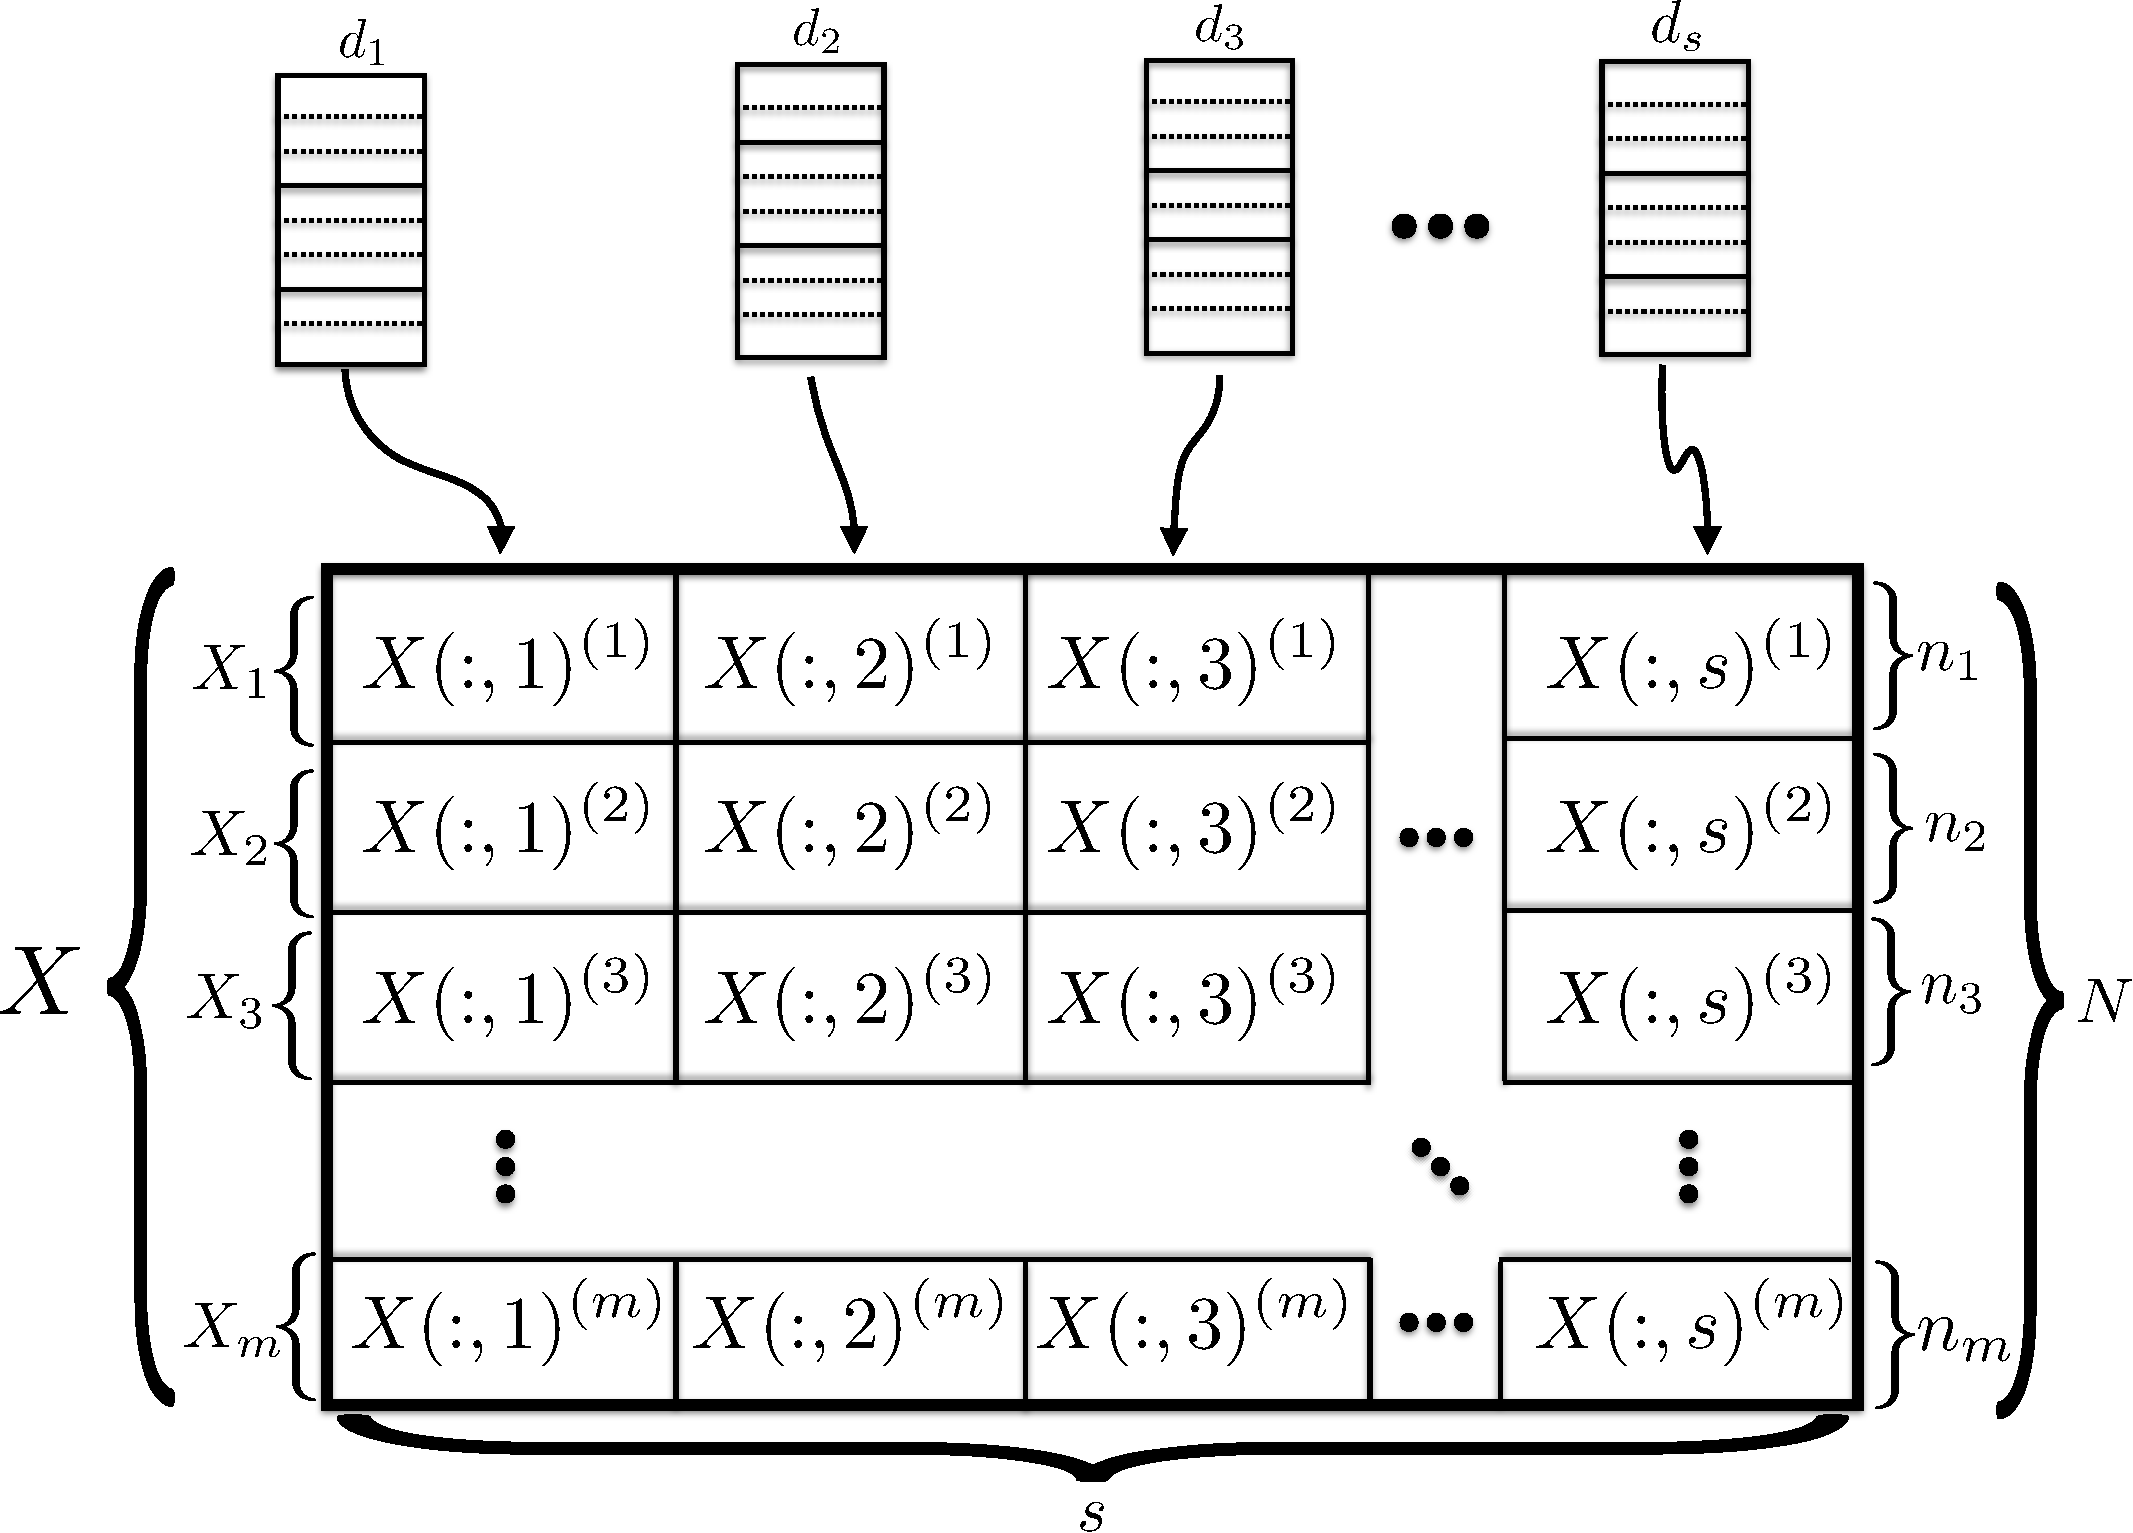
\includegraphics[width=9cm]{figures/stacked_matrices1-crop.pdf}
\caption{\label{fig:stacked_matrices} Multilingual corpora and their matrix representations using the vector space model.}
\end{figure}

We will now describe four models to cross-lingual similarity computation in the next sub-sections.
\section{$k$-means}\label{sec:kmeans}

The $k$-means algorithm is perhaps the most well-known and widely-used clustering algorithm. Here, we present its application
to compute cross-lingual similarities. The idea is based on concatenating the corpus matrices, running standard $k$-means clustering to obtain the matrix of centroids, ``reversing" the concatenation step to obtain a set of aligned bases, which are finally used to compute cross-lingual similarities. See Figure~\ref{fig:kmeans} for overview of the procedure. The left side of Figure~\ref{fig:kmeans} illustrates the decomposition and the right side summarizes the coordinate change.

\begin{figure}[tbp]
\centering
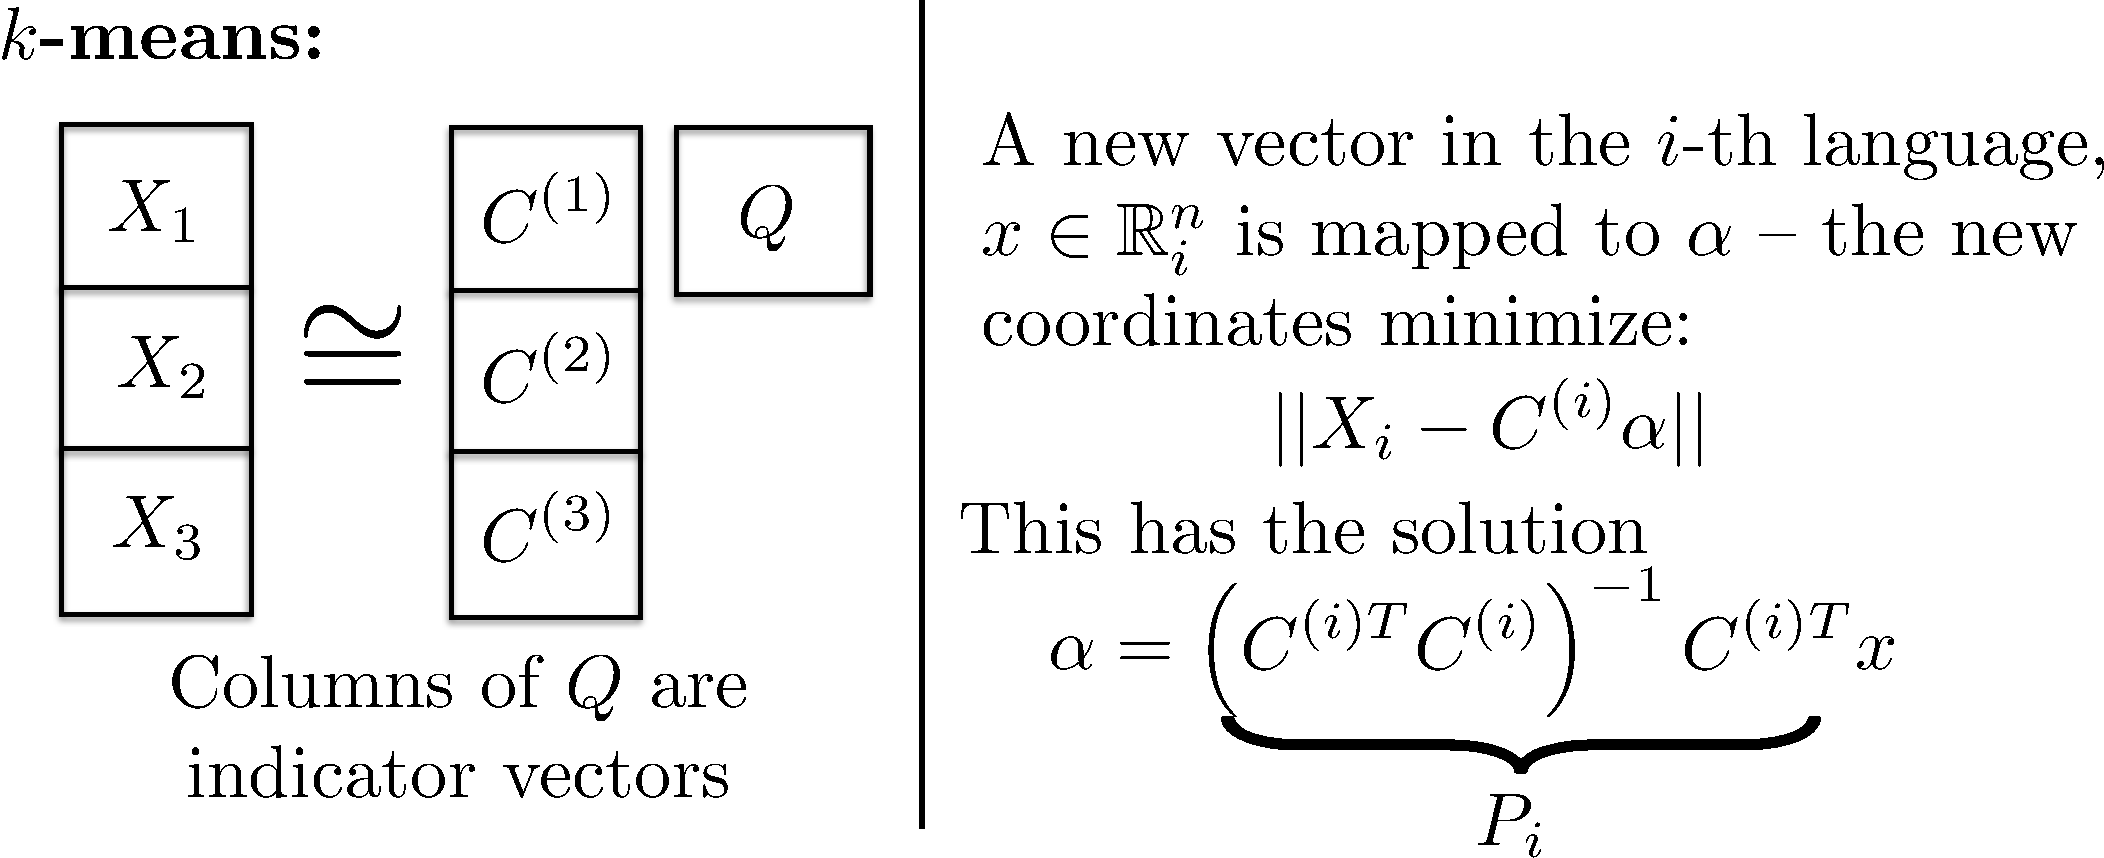
\includegraphics[width=10cm]{figures/kmeans.pdf}
\caption{\label{fig:kmeans} $k$-means algorithm and coordinate change.}
\end{figure}

 In order to apply the algorithm, we first merge all the term-document matrices into a single matrix $X$ by stacking the individual term-document matrices (as seen in Figure~\ref{fig:stacked_matrices}):
$$X := \begin{bmatrix}X_1^T ,X_2^T, \cdots, X_m^T \end{bmatrix}^T,$$
such that the columns respect the alignment of the documents (here MATLAB notation for concatenating matrices is used). Therefore, each document  is represented by a long vector indexed by the terms in all languages.

We then run the $k$-means algorithm~\cite{kmeans} and obtain a centroid matrix $C \in \RR^{N \times k}$, where the $k$ columns represent centroid vectors. The centroid matrix can be split vertically into $m$ blocks: $$C = [C_1^T \cdots C_m^T]^T,$$ according to the number of dimensions of each language, i.e., $C_i \in \RR^{n_i \times k}$.
%
To reiterate, the matrices $C_i$ are computed using a multilingual corpus matrix $X$ (based on Wikipedia for example).

To compute  cross-lingual document similarities on new documents, note that each matrix $C_i$ represents a vector space basis and can be used to map points in $\RR^{n_i}$ into a $k$-dimensional space, where the new coordinates of a vector $x \in \RR^{n_i}$ are expressed as: $$(C_i^T C_i)^{-1} C_i^T x_i.$$

The resulting matrix for similarity computation between language $i$ and language $j$ is defined up to a scaling factor as:
$$C_i(C_i^T C_i)^{-1} (C_j^T C_j)^{-1} C_j.$$

The matrix is a result of mapping documents in a language independent space using pseudo-inverses of the centroid matrices $P_i = (C_i^T C_i)^{-1} C_i$ and then comparing them using the standard inner product, which results in the matrix $P_i^T P_j$. For the sake of presentation, we assumed that the centroid vectors are linearly independent. (An independent subspace could be obtained using an additional Gram-Schmidt step~\cite{golub} on the matrix $C$, if this was not the case.)

\section{Cross-Lingual Latent Semantic Indexing}\label{sec:LSI}

The second approach we consider is Cross-Lingual Latent Semantic Indexing (CL-LSI)~\cite{cl_lsi} which is a variant of LSI~\cite{lsi} for more than one language. The approach is very similar to $k$-means, where we first concatenate the corpus matrices, compute a decomposition, which in case of CL-LSI is a truncated Singular Value Decomposition (SVD), decouple the
 column space matrix and use the blocks to compute linear maps to a common vector space, where standard cosine similarity is used to compare documents.

 The method is based on computing a truncated singular value decomposition of the concatenated corpus matrix $X \approx U S V^T$. See Figure~\ref{fig:lsi} for the decomposition. Representing documents in ``topic`` coordinates is done in the same way as in the $k$-means case (see Figure~\ref{fig:kmeans}), we will describe how to compute the coordinate change functions.

\begin{figure}[tbp]
\centering
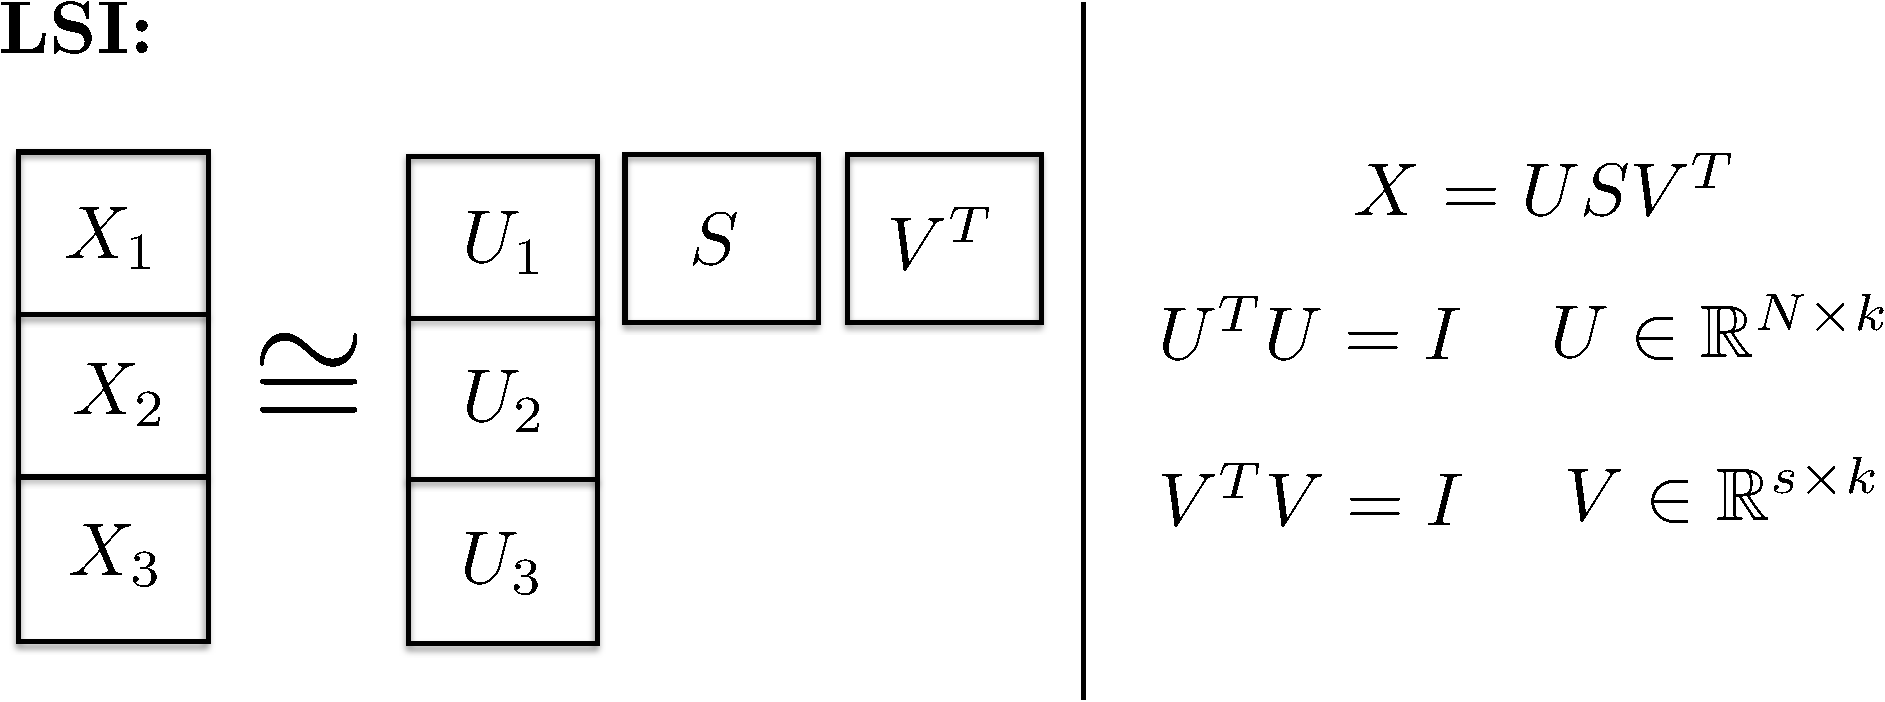
\includegraphics[width=10cm]{figures/lsi.pdf}
\caption{\label{fig:lsi} LSI multilingual corpus matrix decomposition.}
\end{figure}

The cross-lingual similarity functions are based on a rank-$k$ truncated SVD: $X \approx U \Sigma V^T,$ where $U \in \RR^{N \times k}$ are basis vectors of interest and $\Sigma \in \RR^{k \times k}$ is a truncated diagonal matrix of singular eigenvalues. An aligned basis is obtained by first splitting $U$ vertically according to the number of dimensions of each language: $U = [U_1^T \cdots U_m^T]^T$. Then, the same as with $k$-means clustering, we compute the pseudoinverses $P_i = (U_i^T U_i)^{-1} U_i^T$. The matrices $P_i$ are used to change the basis from the standard basis in $\RR^{n_i}$ to the basis spanned by the columns of $U_i$.

\paragraph{Implementation note}

  Since the matrix $X$ can be large we could use an iterative method like the Lanczos algorithm with reorthogonalization~\cite{golub} to find the left singular vectors (columns of $U$) corresponding to the largest singular values. It turns out that the Lanczos method converges slowly as the gap between the leading singular values is small. Moreover, the Lanczos method is hard to parallelize. Instead, we use a randomized version of the SVD~\cite{tropp} that can be viewed as a block Lanczos method. That enables us to use parallelization and speeds up the computation considerably.

To compute the matrices $P_i$ we used the QR algorithm~\cite{golub} to factorize $U_i$ as $U_i = Q_i R_i$, where $Q_i^TQ_i = I$ and $R_i$ is a triangular matrix. $P_i$ is then obtained by solving $R_i P_i = Q_i$.

\section{Canonical Correlation Analysis}\label{sec:CCA}
 We now present a statistical technique to analyze data from two sources, an extension of which will be presented in the next section.
%
 Canonical Correlation Analysis (CCA)~\cite{Hotelling} is a dimensionality reduction technique similar to Principal Component Analysis (PCA)~\cite{Pearson1901On}, with the additional assumption that the data consists of feature vectors that arose from two sources (two views) that share some information. Examples include: bilingual document collection ~\cite{mrpqr} and collection of images and captions~\cite{Hardoon_usingimage}. Instead of looking for linear combinations of features that maximize the variance (PCA) we look for a linear combination of feature vectors from the first view and a linear combination for the second view, that are maximally correlated.

Interpreting the columns of $X_i$ as observation vectors sampled from an underlying distribution $\mathcal{X}_i \in \RR^{n_i}$, the idea is to find two weight vectors $w_i \in \RR^{n_i}$ and $w_j \in \RR^{n_j}$ so that the random variables $w_i^T \cdot \mathcal{X}_i$ and $w_j^T \cdot \mathcal{X}_j$ are maximally correlated ($w_i$ and $w_j$ are used to map the random vectors to random variables, by computing weighted sums of vector components). Let $\rho(x,y)$ denote the sample-based correlation coefficient between two vectors of observations $x$ and $y$. By using the sample matrix notation $X_i$ and $X_j$ (assuming no data is missing to simplify the exposition), this problem can be formulated as the following optimization problem:
\begin{equation*}
\begin{aligned}
& \underset{w_i \in \RR^{n_i}, w_j \in \RR^{n_j}}{\text{maximize}}
& & \rho(w_i^T X_i , w_j^T X_j) = \frac{w_i^T C_{i,j} w_j}{\sqrt{w_i^T C_{i,i} w_i} \sqrt{w_j^T C_{j,j} w_j}},
\end{aligned}
\end{equation*}
where $C_{i,i}$ and $C_{j,j}$ are empirical estimates of variances of $\mathcal{X}_i$ and $\mathcal{X}_j$ respectively and $C_{i,j}$ is an estimate for the covariance matrix. Assuming that the observation vectors are centered (only for the purposes of presentation), the matrices are computed in the following way: $C_{i,j} = \frac{1}{n-1}X_i X_j^T$, and similarly for $C_{i,i}$ and $C_{j,j}$.
The optimization problem can be reduced to an eigenvalue problem and includes inverting the variance matrices $C_{i,i}$ and $C_{j,j}$. If the matrices are not invertible, one can use a regularization technique by replacing $C_{i,i}$ with $(1- \kappa)C_{i,i} + \kappa I$, where $\kappa \in [0,1]$ is the regularization coefficient and $I$ is the identity matrix. (The same can be applied to $C_{j,j}$.)
A single canonical variable is usually inadequate in representing the original random vector and typically one looks for $k$ projection pairs $(w_i^1, w_j^1),\ldots,(w_i^k, w_j^k)$, so that $(w_i^{u})^T \mathcal{X}_i$ and $(w_j^{u})^T \mathcal{X}_j$ are highly correlated and $(w_i^{u})^T \mathcal{X}_i$ is uncorrelated with $(w_i^{v})^T \mathcal{X}_i$  for $u \neq v$ and analogously for $w_j^u$ vectors.

Note that the method in its original form is only applicable to two languages where an aligned set of observations is available. The next section will describe a scalable extension of CCA to more than two languages.

\section{Hub language based CCA Extension}\label{sec:hublang}
Building cross-lingual similarity models based on comparable corpora is challenging for two main reasons. The first problem is related to missing alignment data: when a number of languages is large, the dataset of documents that cover all languages is small (or may even be empty). Even if only two languages are considered, the set of aligned documents can be small (an extreme example is given by the Piedmontese and Hindi Wikipedias where no inter-language links are available), in which case none of the methods presented so far are applicable.
 The second challenge is scale - the data is high-dimensional (many languages with hundreds of thousands of features per language) and the number of multilingual documents may be large (over one million in case of Wikipedia). The optimization problem posed by CCA is not
 trivial to solve: the covariance matrices themselves are prohibitively large to fit in memory (even storing a 100,000 by 100,000 element matrix requires 80GB of memory) and iterative matrix-multiplication based approaches to  solving generalized eigenvalue problems are required (the covariance matrices can be expressed as products of sparse matrices, which means we have fast matrix-vector multiplication).

We now describe an extension of CCA to more than two languages, which can be trained on large comparable corpora and can handle missing data.
 The extension we consider is based on a generalization of CCA to more than two views, introduced in~\cite{Kettenring}, namely the Sum of Squared Correlations SSCOR, which we will state formally later in this section. Our approach exploits a certain characteristic of the data, namely the \emph{hub language} characteristic (see below) in two
 ways: to reduce the dimensionality of the data and to simplify the optimization problem.

\paragraph{Hub language characteristic.}
In the case of Wikipedia, we observed that even though the training resources are scarce for certain language pairs, there often exists indirect training data. By considering a third language, which has training data with both languages in the pair,  we can use the composition of learned maps as a proxy. We refer to this third language as a hub language.

A \emph{hub language} is a language with a high proportion of non-empty documents in $D = \left\{d_1,..., d_{\ell}\right\}$. As we have mentioned, we only focus on multilingual documents that include at least two languages. The prototypical example in the case of Wikipedia is English. Our notion of the hub language could be interpreted in the following way.
If a non-English Wikipedia page contains one or more links to variants of the page in other languages, English is very likely to be one of them. That makes English a hub language.

We use the following notation to define subsets of the multilingual comparable corpus: let $a(i,j)$ denote the index set of all multilingual documents with non-missing data for the $i$-th and $j$-th language:  $$a(i,j) = \left\{k~ |~ d_k = (u_1,...,u_m), u_i \neq \emptyset, u_j \neq \emptyset \right\},$$ and let $a(i)$ denote the index set of all multilingual documents with non missing data for the $i$-th language.

We now describe a two step approach to building a cross-lingual similarity matrix. The first part is related to LSI and reduces the dimensionality of the data. The second step refines the linear mappings and optimizes the linear dependence between data.

\paragraph{Step 1: Hub language based dimensionality reduction.}

The first step in our method is to project $X_1, \ldots, X_m$ to lower-dimensional spaces without destroying the cross-lingual structure. Treating the nonzero columns of $X_i$ as observation vectors sampled from an underlying distribution $\mathcal{X}_i \in V_i = \RR^{n_i}$, we can analyze the empirical cross-covariance matrices:
$$C_{i,j} = \frac{1}{|a(i,j)|-1 }\sum_{\ell \in a(i,j)} (X_i^{\ell} - c_i)\cdot (X_j^{\ell} - c_j)^T,$$
 where $c_i = \frac{1}{a_i} \sum_{\ell \in a(i)}X_i^{\ell}$. By finding low-rank approximations of $C_{i,j}$ we can identify the subspaces of $V_i$ and $V_j$ that are relevant for extracting linear patterns between $\mathcal{X}_i$ and $\mathcal{X}_j$. Let $X_1$ represent the hub language corpus matrix. The LSI approach to finding the subspaces is to perform the singular value decomposition on the full $N \times N$ covariance matrix composed of blocks $C_{i,j}$. If $|a(i,j)|$ is small for many language pairs (as it is in the case of Wikipedia), then many empirical estimates $C_{i,j}$ are unreliable, which can result in overfitting. For this reason, we perform the truncated singular value decomposition on the matrix $C = [C_{1,2}  \cdots  C_{1,m}] \approx U S V^T$, where $U \in \RR^{n_1 \times k}, S \in \RR^{k \times k}, V \in \RR^{(\sum_{i=2}^m n_i) \times k}$. We split the matrix $V$ vertically in blocks with $n_2, \ldots, n_m$ rows: $V = [V_2^T  \cdots  V_m^T]^T$. Note that columns of $U$ are orthogonal but columns in each $V_i$ are not (columns of V are orthogonal). Let $V_1 := U$. We proceed by reducing the dimensionality of each $X_i$ by setting: $Y_i = V_i^T \cdot X_i$, where $Y_i \in \RR^{k\times N}$. To summarize, the first step reduces the dimensionality of the data and is based on CL-LSI, but optimizes only the hub language related cross-covariance blocks.

\paragraph{Step 2: Simplifying and solving SSCOR.}
The second step involves solving a generalized version of canonical correlation analysis on the matrices $Y_i$ in order to find the mappings $P_i$. The approach is based on the sum of squares of correlations formulation by Kettenring~\cite{Kettenring}, where we consider only correlations between pairs $(Y_1, Y_i), i >1$ due to the hub language problem characteristic.
We will present the original unconstrained optimization problem, then a constrained formulation based on the hub language problem characteristic. Then we will simplify the constraints and reformulate the problem as an eigenvalue problem by using Lagrange multipliers.

The original sum of squared correlations is formulated as an unconstrained problem:
\begin{equation*}
  \begin{aligned}
    & \underset{w_i \in \RR^{k}}{\text{maximize}}
    & & \sum_{i < j}^m  \rho(w_i^T Y_i, w_j^T Y_j)^2.
\end{aligned}
\end{equation*}
We solve a similar problem by restricting $i=1$ and omitting the optimization over non-hub language pairs.
Let $D_{i,i} \in \RR^{k \times k}$ denote the empirical covariance of $\mathcal{Y}_i$ and $D_{i,j}$ denote the empirical cross-covariance computed based on $\mathcal{Y}_i$ and $\mathcal{Y}_j$. We solve the following constrained (unit variance constraints) optimization problem:
\begin{equation}\label{squaredCorHubOriginal}
  \begin{aligned}
    & \underset{w_i \in \RR^{k}}{\text{maximize}}
    & & \sum_{i = 2}^m  \left(w_1^T D_{1,i} w_i \right)^2
    & \text{subject to}
    & & w_i^T D_{i,i} w_i = 1, \quad\forall i = 1,\ldots, m.
\end{aligned}
\end{equation}
The constraints $w_i^T D_{i,i} w_i$ can be simplified by using the Cholesky decomposition $D_{i,i} = K_i^T \cdot K_i$ and substitution: $y_i := K_i w_i$. By inverting the $K_i$ matrices and defining  $G_i := K_1^{-T} D_{1,i} K_i^{-1}$, the problem can be reformulated:
\begin{equation}\label{squaredCorHub}
  \begin{aligned}
    & \underset{y_i \in \RR^{k}}{\text{maximize}}
    & & \sum_{i = 2}^m  \left(y_1^T G_{i} y_i \right)^2
    & \text{subject to}
    & & y_i^T y_i = 1, \quad\forall i = 1,\ldots, m.
\end{aligned}
\end{equation}
A necessary condition for optimality is that the derivatives of the Lagrangian vanish. The Lagrangian of (\ref{squaredCorHub}) is expressed as:
$$  L(y_1, \ldots, y_m, \lambda_1, \ldots, \lambda_m) = \sum_{i = 2}^m  \left(y_1^T G_{i} y_i \right)^2 + \sum_{i=1}^m \lambda_i \left(y_i^T y_i - 1\right).$$
Stationarity conditions give us:
\begin{equation}\label{dLdx1}
 \frac{\partial}{\partial x_1} L = 0 \Rightarrow \sum_{i = 2}^m  \left(y_1^T G_{i} y_i \right) G_i y_i + \lambda_1 y_1 = 0,
\end{equation}
\begin{equation}\label{dLdxi}
\frac{\partial}{\partial x_i} L = 0 \Rightarrow \left(y_1^T G_{i} y_i \right) G_{i}^T y_1 + \lambda_i y_i = 0,~i > 1.
\end{equation}
Multiplying the equations (\ref{dLdxi}) with $y_i^T$ and applying the constraints, we can eliminate $\lambda_i$ which gives us:
\begin{equation}\label{eqy1yi}
G_{i}^T y_1 = \left(y_1^T G_{i} y_i \right) y_i,~i > 1.
\end{equation}
Plugging this into (\ref{dLdx1}), we obtain an eigenvalue problem:
$$\left( \sum_{i = 2}^m G_i G_{i}^T \right) y_1 + \lambda_1 y_1 = 0.$$
The eigenvectors of $\left( \sum_{i = 2}^m G_i G_{i}^T \right)$ solve the problem for the first language. The solutions for $y_i$ are obtained from (\ref{eqy1yi}): $y_i := \frac{G_{i}^T y_1}{\| G_{i}^T y_1 \|}$.
Note that the solution (\ref{squaredCorHubOriginal}) can be recovered by: $w_i := K_i^{-1} y_i$. The linear transformation of the $w$ variables are thus expressed as:
$$ Y_1 := \text{eigenvectors of} \sum_{i = 2}^m G_i G_{i}^T, $$
$$ W_1 = K_1^{-1} Y_1 $$
$$ W_i = K_i^{-1} G_{i}^T Y_1 N,$$
where $N$ is a diagonal matrix that normalizes $G_{i}^T Y_1$, with $N(j,j) := \frac{1}{\|G(_{i} Y_1(:,j)\|}$.

\paragraph{Remark.} The technique is related to  Generalization of Canonical Correlation Analysis (GCCA) by Carroll~\citeyear{Carroll}, where an unknown group configuration variable is defined and the objective is to maximize the sum of squared correlations between the group variable and the others. The problem can be reformulated as an eigenvalue problem. The difference lies in the fact that we set the unknown group configuration variable as the hub language, which simplifies the solution. The complexity of our method is $O(k^3)$, where $k$ is the reduced dimension from the LSI preprocessing step, whereas solving the GCCA method scales as $O(s^3)$, where $s$ is the number of samples (see~\cite{gifi}). Another issue with GCCA is that it cannot be directly applied to the case of missing documents.

To summarize, we first reduced the dimensionality of our data to $k$-dimensional features and then found a new representation (via linear transformation) that maximizes directions of linear dependence between the languages. The final projections that enable mappings to a common space are defined as: $P_i(x) = W_i^T V_i^T x.$


%
% Sixth chapter
%--------------------------------------------------------------------------------------------------
%
\chapter{Experiments}
%--------------------------------------------------------------------------------------------------



\vspace{-0.1cm}
\section{Experiments}\label{sec:experiments}

We evaluated the local and global approaches on two scenarios: a performance
analysis on synthetic data and the performance on finding a common
representation of a cross-lingual collection of documents.
%, performance of the methods on the task of signal blind source separation and an exploratory analysis of sensor network data.

\subsection{Synthetic data}\label{subsec:syndata}
We generated several MCCA problem instances by varying the number
of views and number the of dimensions per view in order to
compare the performance of local search methods and the proposed
SDP relaxation. The goal of these experiments was to see
under which conditions and how often do the global bounds
provide useful information.

 Let $m$ denote the number of views
(sets of variables) and $n_i$ denote the dimensionality of $i$-th
view and $N := \sum_i n_i$. In all cases, we used the same number
of dimensions per view ($n_1 = n_2 = \cdots = n_m$). We used
three different methods to generate random correlation matrices.

The first method,  the \textbf{random Gram matrices} method (see
\cite{Holmes:1991:RCM:105724.105730}, \cite{Bendel_Mickey_78}) ,
generates the correlation matrices by sampling $N$ vectors $v_1,
\ldots, v_n$ for an $N$-dimensional multivariate Gaussian
distribution (centered at the origin, with an identity covariance
matrix), normalizing them and computing the correlation matrix $C
= \left[c_{i,j}\right]_{N \times N}$ as $c_{i,j} := v_i' \cdot v_j$.
%
The second method,  the \textbf{random spectrum} method,
samples the eigenvalues $\lambda_1,\ldots,\lambda_N$ uniformly
from a simplex ($\sum_{i=1}^{N} \lambda_i = N$) and generates a
random correlation matrix with the prescribed eigenvalues (see
\cite{Bendel_Mickey_78}).
%
The final method, the \textbf{random 1-dim structures} method,
generates a correlation matrix that has an approximately (due to
noise) single-dimensional correlation structure. We
generate a random $m$ dimensional Gram matrix $B$, and insert
it into an $N\times N$ identity matrix according to the block
structure to obtain a matrix $C_0$. That is, we set $C_0\left(i,j\right) = \delta\left(i,j\right)$,
where $\delta$ is the Kronecker delta. For $I,J = 1\ldots,m$, we
override the entries $$C_0\left(1+ \sum_{i=1}^{I-1}n_i, 1+
\sum_{i=1}^{J-1}n_i\right) = B\left(I,J\right),$$ where we used $1$-based
indexing. We then generate a random Gram matrix $D \in
\RR^{N\times N}$ and compute the final correlation matrix as $C
= \left(1- \epsilon\right)C_0 + \epsilon D$.
 In our experiments, we set
$\epsilon = 0.001$.

The purpose of using a random spectrum method
is that as the dimensionality increases, random vectors tend to
be orthogonal, hence the experiments based on random Gram
matrices might be less informative. As the experiments show, the
local method suffers  when all $n_i = 1$ (an
instance of a BQO problem). By using the approximately
1-dimensional correlation matrix sampling, we investigated how the
problem behaves when $n_i > 1$.
%
In all cases, we perform a final step that involves computing the
per-view Cholesky decompositions of variances and change of basis
%as we showed when we arrived to QCQP reformulation in equation
(as in \ref{eq:qcqp}).


The experiments are based on varying the number of sets of
variables, $m$ and the dimensionality $n_i$. For each sampling
scenario and each choice of $m$ and $n_i$, we generated $100$
experiments, and computed $1000$ solutions based on Algorithm
\ref{algorithm:horst},  the SDP solution (and respective
global bounds), and examined the frequencies of the following
events:
\begin{itemize}
\item a \textbf{duality gap} candidate detected (Tables
\ref{tb:rg}, \ref{tb:rs}, \ref{tb:r1d} (a))
\item \textbf{local convergence} detected (Tables \ref{tb:rg}, \ref{tb:rs},
\ref{tb:r1d} (b))
\item when a local solution is worse
than the SDP-based \textbf{lower bound} (Tables \ref{tb:rg},
\ref{tb:rs}, \ref{tb:r1d} (c)).
\end{itemize}
The possibility of a duality gap is
detected when the best local solution is lower than $1\%$ of the
SDP bound. In this case, the event indicates only the possibility
of duality gap -- it might be the case that further local
algorithm restarts would close the gap. Local convergence
is detected when the objective value of two local solutions
differs relatively by at least $10\%$ and absolutely at least by
$0.1$ (both criteria must be satisfied
simultaneously). Finally, the event of a local solution being
below the SDP lower bound means that it is below
$\frac{2}{\pi}$ of the optimal objective value of the SDP
relaxation.

We find that regardless of the generation technique, the lower
SDP bound is useful only when $n_i = 1$ (Table \ref{tb:rg},
\ref{tb:rs}, \ref{tb:r1d} (c)) and the results are similar for
different choices of $m$. There are, however rare instances (less
than $0.1\%$) where the lower bound is useful for $n_i = 2$ and
even rarer (less than $0.01\%$) for $n_i = 3$.

The chance of local convergence increases as the number of views
$m$ increases which can be consistently observed for all choices
of $n_i$ and sampling strategies. Generating a generic  problem where the
local algorithm  converges to a local solution is less
likely as the dimensionality increases
(Tables \ref{tb:rg}, \ref{tb:rs}).
%
%
%\textcolor{red}{Nasledni odstavek ne razumem}
%\textcolor{red}{Sem popravil. A je OK? Jan}
In the case of noisy embeddings of a 1-dimensional correlation structures, the dependence on $n_i$
behaves differently: the local convergence (see Table \ref{tb:r1d_lc}) for the case $\left(m=5, n_i=3\right)$ is more likely than for the case $\left(m=5, n_i =2\right)$. This is unexpected as in the general case, increasing $n_i$ reduces that chance of local convergence, see Table \ref{tb:rs_lc}, Table \ref{tb:rg_lc}.

The relationship between $m$ and $n_i$ and the possibility of a
duality gap behaves similarly as local convergence -
increasing $m$ increases it and increasing $n_i$ decreases it (Table \ref{tb:rg_dg}, Table \ref{tb:rs_dg}),
except in the case of noisy 1-dim correlation structures, where
we observe the same anomaly when $n_i = 2$ (Table \ref{tb:r1d_dg}).

Therefore we have demonstrated that there exist sets of problems with nonzero
measure where the SDP bounds give useful information.
%
%\begin{table}
%\begin{center}
%\caption{\label{tb:rg} Random Gram matrix sampling}
%\subtable[Possible duality gap]{\label{tb:rg_dg}
%\centering\begin{tabular}{|l|c|c|c|}
\hline
&\textbf{$n_i$ = 3}&\textbf{$n_i$ = 2}&\textbf{$n_i$ = 1}\\\hline
\textbf{$m$ = 5}&0\%&5\%&17\%\\\hline
\textbf{$m$ = 3}&0\%&0\%&9\%\\\hline
\end{tabular}

%}
%\subtable[Local convergence]{\label{tb:rg_lc}
%\centering\begin{tabular}{|l|c|c|c|}
\hline
&\textbf{$n_i$ = 3}&\textbf{$n_i$ = 2}&\textbf{$n_i$ = 1}\\\hline
\textbf{$m$ = 5}&1\%&5\%&48\%\\\hline
\textbf{$m$ = 3}&0\%&1\%&26\%\\\hline
\end{tabular}

%}
%\subtable[Local solution below lower SDP bound]{\label{tb:rg_lb}
%\centering\begin{tabular}{|l|c|c|c|}
\hline
&\textbf{$n_i$ = 3}&\textbf{$n_i$ = 2}&\textbf{$n_i$ = 1}\\\hline
\textbf{$m$ = 5}&0\%&0\%&14\%\\\hline
\textbf{$m$ = 3}&0\%&0\%&12\%\\\hline
\end{tabular}

%}%
%\end{center}
%\end{table}
%%
%\begin{table}
%\begin{center}
%\caption{\label{tb:rs}Random spectrum sampling}
%\subtable[Possible duality gap]{\label{tb:rs_dg}
%\centering\begin{tabular}{|l|c|c|c|}
\hline
&\textbf{$n_i$ = 3}&\textbf{$n_i$ = 2}&\textbf{$n_i$ = 1}\\\hline
\textbf{$m$ = 5}&0\%&5\%&36\%\\\hline
\textbf{$m$ = 3}&0\%&1\%&20\%\\\hline
\end{tabular}

%}
%\subtable[Local convergence]{\label{tb:rs_lc}
%\centering\begin{tabular}{|l|c|c|c|}
\hline
&\textbf{$n_i$ = 3}&\textbf{$n_i$ = 2}&\textbf{$n_i$ = 1}\\\hline
\textbf{$m$ = 5}&1\%&3\%&50\%\\\hline
\textbf{$m$ = 3}&0\%&0\%&31\%\\\hline
\end{tabular}

%}
%\subtable[Local solution below lower SDP bound]{\label{tb:rs_lb}
%\centering\begin{tabular}{|l|c|c|c|}
\hline
&\textbf{$n_i$ = 3}&\textbf{$n_i$ = 2}&\textbf{$n_i$ = 1}\\\hline
\textbf{$m$ = 5}&0\%&0\%&15\%\\\hline
\textbf{$m$ = 3}&0\%&0\%&16\%\\\hline
\end{tabular}

%}%
%\end{center}
%\end{table}
%%
%\begin{table}
%\begin{center}
%\caption{\label{tb:r1d}Random 1-dim structure sampling}
%\subtable[Possible duality gap]{\label{tb:r1d_dg}
%\centering\begin{tabular}{|l|c|c|c|}
\hline
&\textbf{$n_i$ = 3}&\textbf{$n_i$ = 2}&\textbf{$n_i$ = 1}\\\hline
\textbf{$m$ = 5}&24\%&16\%&23\%\\\hline
\textbf{$m$ = 3}&7\%&4\%&7\%\\\hline
\end{tabular}

%}
%\subtable[Local convergence]{\label{tb:r1d_lc}
%\centering\begin{tabular}{|l|c|c|c|}
\hline
&\textbf{$n_i$ = 3}&\textbf{$n_i$ = 2}&\textbf{$n_i$ = 1}\\\hline
\textbf{$m$ = 5}&9\%&6\%&51\%\\\hline
\textbf{$m$ = 3}&0\%&0\%&31\%\\\hline
\end{tabular}

%}
%\subtable[Local solution below lower SDP bound]{\label{tb:r1d_lb}
%\centering\begin{tabular}{|l|c|c|c|}
\hline
&\textbf{$n_i$ = 3}&\textbf{$n_i$ = 2}&\textbf{$n_i$ = 1}\\\hline
\textbf{$m$ = 5}&0\%&0\%&13\%\\\hline
\textbf{$m$ = 3}&0\%&0\%&15\%\\\hline
\end{tabular}

%}%
%\end{center}
%\end{table}


\subsection{Multilingual document collection}\label{subsec:documents}
%\textbf{Motivation}

Applications of canonical correlation analysis on collections of
documents include: dimensionality reduction, cross-lingual document retrieval and classification
\cite{ccatext} \cite{ccatextdva}, multilingual topic extraction
 \cite{mcca} and news bias detection \cite{ccanewsbias}. In this section, we explore the behavior of
Algorithm \ref{algorithm:horst} with respect to the global
bounds on real data. We start by describing the data and then describe a method to
reduce the dimensionality of the data in order to apply the SDP
bounds.


\noindent\textbf{Dataset and preprocessing}
The experiments were conducted on a subset of EuroParl, Release v3,
\cite{europarl}, a multilingual parallel corpus, where our subset
includes Danish, German, English, Spanish, Italian, Dutch,
Portuguese and Swedish. We first removed all documents
which had one translation or more missing. Documents (each
document is a day of sessions of the parliament) were then
arranged alphabetically and split into smaller documents, such that
each speaker instance represented a separate document.
Therefore, we ended up with $12,000$ documents per
language. These roughly correspond to all speeches between 2.25.1999
and 3.25.1999. We then computed the bag of words (vector space)
\cite{Salton88term-weightingapproaches} model for each language,
keeping unigrams, bigrams and trigrams that occurred
more than thirty times.
%For example: "Mr", "President" and
%"Mr\_President" all occurred more than thirty times in the
%English part of the corpus and they each represent a dimension in
%the vector space.
This resulted in feature spaces with
dimensionality ranging from $50,000$ (English) to $150,000$
(German). Finally, we computed the tf-idf weighting and normalized
every document for each language. Therefore, we obtained
corpus matrices $X^{(i)}$ for each language, where each
matrix has $12,000$ columns and the columns are aligned
($X^{(i)}\left(:,\ell\right)$ and $X^{(j)}\left(:,\ell\right)$ are a translation of
each other). %In section \ref{sec:sumcorextensions} we showed how to
%derive the QCQP problem, given a set of input matrices $X^{(i)}$.

\noindent\textbf{Random projections and multivariate regression}
%experiments: languagesSDP_main
Applying the global (SDP) techniques to these covariance matrices
presents a scalability problem,  both from the large number
of features (words in vocabulary) and the large number of documents. Typical SDP solvers can find solutions to relaxed forms of
QCQPs with up to a few thousand original variables, which is
insufficient in this case, since the primal representation results in hundreds of thousands of dimensions, and the dual representation results in $25,000$ dimensions (five languages, each containing $5000$ training documents).


 To address this issue,  we
reduce the dimensionality of the feature vectors, resulting in
tractable SDP problem dimensions.
%
One way to analyze a monolingual document collection is to
perform a singular value decomposition of the corpus matrix, a
technique referred to as Latent Semantic Indexing
(LSI)\cite{lsi}. A set of largest singular vectors can be used as
a new document basis for dimensionality reduction. Expressing the
documents with the basis of $k$ largest singular vectors is
optimal with respect to Frobenious norm reconstruction error. If
computing the basis is too expensive, one can generate a random
larger set of basis vectors that achieve similar reconstruction
errors. However, this random projection basis is not
informative in the same sense as the LSI basis is (topics extracted by LSI reflect which topics are
relevant for the corpus, as opposed to random topics).

A variant of LSI for multiple languages, Cross-Lingual LSI
(CL-LSI)\cite{cl_lsi}, first joins all feature spaces thus
obtaining a single multilingual corpus matrix (single language
corpus matrices are stacked together). CL-LSI then proceeds as
standard LSI by computing the singular value decomposition (SVD) of the
multilingual corpus matrix.
%
We experimentally observed that the number
of random projections needed to approximate the decomposition in CL-LSI and thus capture
multi-lingual topics is prohibitively large - while a relatively small number
of random projections is needed to capture the variance in each language, a large
number of random projections is needed to approximate all the cross-covariance matrices simultaneously.
Generating random subspaces with a fixed $k$ sequentially over each language becomes harder with each language.
The probability of generating a subspace for the $m$-th language that is well correlated to the preceding languages decreases
as $m$ increases.

Our approach is based on the following idea. Generate a set of random vectors for one language and use Canonical Correlation Analysis Regression (CCAR)\cite{ccar} (a method similar to ridge regression) to find their representatives in the other languages. Repeat the procedure for each of the remaining languages to prevent bias to a single language. We hypothesize that restricting our search in the spaces spanned by the constructed bases still leads to good solutions. The procedure is detailed in Algorithm \ref{algorithm:rpgen}.

Let $m$ be the number of vector spaces corresponding to different
languages and $n_i$ the dimensionality of the $i-th$ vector
space. Let $X^{(i)} \in \RR^{n_i \times N}$ represent the aligned
document matrix for the $i$-th language.



\begin{algorithm}
\caption{Random projections basis generation}
\label{algorithm:rpgen}
{\bf Input:} $X^{(1)},\ldots X^{(m)}$, $\gamma$ - the regularization coefficient, $k$ - \# of projections/block
\begin{algorithmic}
\FOR{$i = 1$ to $m$}
\STATE $P_{(i,i)} :=$ random $n_i \times k$ matrix with elements sampled $i.i.d.$ from standard normal distribution.
\STATE Re-scale each column of $P_{(i,i)}$ so that its norm is equal to $\sqrt{\frac{n_i}{k}}$.
\FOR{$j = 1$ to $m$}
\IF {$j = i$}
 \STATE continue
\ENDIF
\STATE  $\alpha_{(i,j)} :=  \left(\left(1-\gamma\right) X^{(j)} X^{(j)T} + \gamma  I_j \right)^{-1}$
\STATE  $P_{(i,j)} :=  \alpha_{(i,j)} X^{(j)} X^{(i)T}  P_{(i,i)},$ where $I_j$ is the $n_j \times n_j$ identity matrix.
%\STATE  $P_{(i,j)} :=   \left(\left(1-\gamma\right) X^{(j)} X^{(j)T} + \gamma  I_j \right)^{-1} X^{(j)} X^{(i)T}  P_{(i,i)},$ where $I_j$ is the $n_j \times n_j$ identity matrix.
\ENDFOR
\ENDFOR
\\
\end{algorithmic}
{\bf Output:} matrices $P_{(i,j)} \;\text{for}\; i,j = 1,\ldots,m$
\end{algorithm}

The matrices $P_{(i,1)}, \ldots, P_{(i,m)}$ form the bases of
vector spaces corresponding to $X^{(1)},\ldots, X^{(m)}$. Let
$P_i := \left[P_{(1,i)}, \ldots, P_{(m,i)}\right]$ denote the full basis for
the $i$-th language.
We now experimentally address two questions: does the restricted
space enable us to find \emph{stable patterns} and how informative the SDP
bounds are. Stable patterns are represented by highly correlated directions
in both the training and in independent test sets.

%languagesSDP
%languagesSDP_main
%languageSDP339256474618

%languagesSDP_main(5000, 5, 50, 1000);
%      regprimalS: [0.0100 0.1000 0.5000 0.9000 0.9900]
%     ranprojregS: [0.1000 0.5000 0.9000 0.9900]
%            nexp: 10
%    ntrainPrimal: 5000
%      ntrainDual: 30
%           nview: 5
%        nranproj: 50
%        testsize: 1000
%      resultName: 'languageSDP339256474618'


\noindent\textbf{Experiments}
 The experiments were conducted on the set of five EuroParl
 languages: English, Spanish, German, Italian and Dutch. We set
 $k = 10$ which corresponds to $n_i = 50$ dimensions per view, so
 the QCQP matrix will be of size $250 \times 250$. We randomly
 select $5000$ training documents and $1000$ test documents.  For
 a range of random projection regularization parameters $\gamma$,
 we compute the mappings $P_i$ (based on the train set) and
 reduce the dimensionality of the train and test sets. Then, for
 a range of QCQP regularization parameters $\kappa$, we set up the
 QCQP problem, compute $1000$ local solutions (by Horst
 algorithm) and solve the SDP relaxation. The whole procedure is
 repeated $10$ times.

For each $(\gamma, \kappa)$ pair, we measured the sum of
correlations on the test and train sets. Table
\ref{tb:textTrainTestSumcor} shows the sums of correlations
averaged over $10$ experimental trials. The maximal possible sum
of correlations for five datasets is $\binom{5}{2} = 10$.
We observe that regularizing the whole optimization problem is
not as vital as regularizing the construction of random
projection vectors. This is to be expected since finding the
random projection vectors involves a regression in a high
dimensional space as opposed to solving a lower dimensional
QCQP. Selecting $\gamma = 0.1$ leads to perfectly correlated
solutions on the training set for all $\kappa$. This turns out to
be over-fitted when we evaluate the sum of correlations on the
test set - perfect correlations on the training set turn out to be spurious patterns, since they are not present in the test set.
%The test set does not reflect them (sum of correlations ranges between $5.8$ and $7.4$).
Note that higher $\kappa$ values improve the
performance on the test set up to a certain level below
$7.5$. As we increase $\gamma$ to $0.5$, we see a reduction in
overfitting and with $\gamma = 0.9$ we observe stable patterns. Therefore, using
appropriate values, we can reduce the dimensionality of the
original QCQP problem  and still find stable
solutions.  The reduced dimensionality now enables us to investigate
the behavior of the SDP relaxation.
%
For the SDP bounds, we observed behavior that was similar to the high-dimensional synthetic (generic) case. That is
we found that the potential duality gap was very small and that the SDP and the Horst algorithm yielded the same
result. For this reason we omit the SDP results from Table \ref{tb:textTrainTestSumcor}.

%\begin{table}[tbp]
%\begin{center}
%\caption{\label{tb:textTrainTestSumcor} Train and test sum of correlation}
%\subtable[Train set sum of correlations]{\label{tb:trainText}
%\centering\begin{tabular}{|l|c|c|c|c|}
\hline
&\textbf{$\gamma =$0.1}&\textbf{$\gamma =$0.5}&\textbf{$\gamma =$0.9}&\textbf{$\gamma =$0.99}\\\hline
\textbf{$\kappa =$0.01}&10.0&9.8&9.8&9.8\\\hline
\textbf{$\kappa =$0.1}&10.0&9.8&9.8&9.8\\\hline
\textbf{$\kappa =$0.5}&10.0&9.8&9.8&9.8\\\hline
\textbf{$\kappa =$0.9}&10.0&9.8&9.8&9.8\\\hline
\textbf{$\kappa =$0.99}&10.0&9.8&9.7&9.8\\\hline
\end{tabular}

%}
%\subtable[Test set sum of correlations]{\label{tb:testText}
%\centering\begin{tabular}{|l|c|c|c|c|}
\hline
&\textbf{$\gamma =$0.1}&\textbf{$\gamma =$0.5}&\textbf{$\gamma =$0.9}&\textbf{$\gamma =$0.99}\\\hline
\textbf{$\kappa =$0.01}&5.8&8.6&9.6&9.8\\\hline
\textbf{$\kappa =$0.1}&6.2&8.6&9.6&9.8\\\hline
\textbf{$\kappa =$0.5}&7.0&8.6&9.6&9.8\\\hline
\textbf{$\kappa =$0.9}&7.4&8.8&9.6&9.8\\\hline
\textbf{$\kappa =$0.99}&7.4&8.8&9.6&9.8\\\hline
\end{tabular}

%}
%\end{center}
%\end{table}


\section{Evaluation}\label{sec:evaluation}

We will describe the main dataset for building cross-lingual models which is based on Wikipedia and then present two sets of experiments. The first set of experiments
establishes that the hub based approach can deal with language pairs where little or no training data is available. The second set of experiments compares the main approaches
that we presented on the task of mate retrieval and the task of event linking. Finally, we examine how different choices of features impact the event linking performance.

\subsection{Wikipedia Comparable Corpus}

To investigate the empirical performance of the low-rank approximations we will test the algorithms on a large-scale, real-world multilingual dataset that we extracted from Wikipedia by using inter-language links for alignment. This  results in a large number of weakly comparable documents in more than $200$ languages. Wikipedia is a large source of multilingual data that is especially important for the languages for which no translation tools, multilingual dictionaries as Eurovoc~\cite{eurovoc}, or strongly aligned multilingual corpora as Europarl~\cite{europarl} are available. Documents in different languages are related with so called 'inter-language' links that can be found on the left of the Wikipedia page. The Wikipedia is constantly growing. There are currently 12 Wikipedias with more than 1 million %$10^6$
 articles, $52$ with more than 100k %$10^5$
 articles, $129$ with more than 10k articles, and $236$ with more than $1,000$ articles.

Each Wikipedia page is embedded in the page tag. First, we check if the title of the page starts with a Wikipedia namespace (which includes categories and discussion pages) and do not process the page if it does. Then, we check if this is a redirection page and we store the redirect link because inter-language links can point to redirection links also. If none of the above applies, we extract the text and parse the Wikipedia markup. Currently, all the markup is removed.

We get inter-language link matrix using previously stored redirection links and inter-language links. If an inter-language link points to the redirection we replace it with the redirection target link. It turns out that we obtain the matrix $M$ that is not symmetric, consequently the underlying graph is not symmetric. That means that existence of the inter-language link in one way (i.e., English to German) does not guarantee that there is an inter-language link in the reverse direction (German to English). To correct this we transform this matrix to be symmetric by computing $M+M^T$ and obtaining an undirected graph. In the rare case that after symmetrization we have multiple links pointing from the document, we pick the first one that we encountered. This matrix enables us to build an alignment across all Wikipedia\footnote{https://www.wikipedia.org/ dumps available in 2013} languages.

\subsection{Experiments With Missing Alignment Data}\label{experiments:hubcca}

 In this subsection, we will investigate the empirical performance of hub CCA approach. We will demonstrate that this approach can be successfully applied even in the case of fully missing alignment information.
 To this purpose, we select a subset of Wikipedia languages containing three major languages, English (4,212k articles)--\emph{en} (hub language), Spanish (9,686k articles)--\emph{es}, Russian (9,662k articles)--\emph{ru}, and five minority (in terms of Wikipedia sizes) languages, Slovenian (136k articles)--\emph{sl}, Piedmontese (59k articles)--\emph{pms}, Waray-Waray (112k articles)--\emph{war} (all with about 2 million native speakers), Creole (54k articles)--\emph{ht} (8 million native speakers), and Hindi (97k articles)--\emph{hi} (180 million native speakers). For preprocessing, we remove the documents that contain less than 20 different words (referred to as stubs\footnote{Such documents are typically of low value as a linguistic resource. Examples include the titles of the columns in the table, remains of the parsing process, or Wikipedia articles with very little or no information contained in one or two sentences.}) and remove words occurring in less than 50 documents as well as the top 100 most frequent words (in each language separately). We represent the documents as normalized TFIDF~\cite{Salton88term-weightingapproaches} weighted vectors. The IDF scores are computed for each language based on its aligned documents with the English Wikipedia. The English language IDF scores are based on all English documents for which aligned Spanish documents exist.

The evaluation is based on splitting the data into training and test sets. %(which are described later).
We select the test set documents as all multilingual documents with at least one nonempty alignment from the list: (\emph{hi}, \emph{ht}), (\emph{hi}, \emph{pms}), (\emph{war}, \emph{ht}), (\emph{war}, \emph{pms}). This guarantees that we cover all the languages. Moreover this test set is suitable for testing the retrieval through the hub as the chosen pairs have empty alignments. The remaining documents are used for training. In Table \ref{table:train_test}, we display the corresponding sizes of training and test documents for each language pair.

On the training set, we perform the two step procedure to obtain the common document representation as a set of mappings $P_i$. A test set for each language pair, $test_{i,j} = \{(x_\ell,y_\ell) | \ell = 1:n(i,j)\} $, consists of comparable document pairs (linked Wikipedia pages), where $n(i,j)$ is the test set size. We evaluate the representation by measuring mate retrieval quality on the test sets: for each $\ell$, we rank the projected documents $P_j(y_1),\ldots, P_j(y_{n(i,j)})$ according to their similarity with $P_i(x_\ell)$ and compute the rank of the mate document $r(\ell) = rank(P_j(y_\ell))$. The final retrieval score (between -100 and 100) is computed as: $\frac{100}{n(i,j)} \cdot \sum_{\ell = 1}^{n(i,j)} \left( \frac{n(i,j) - r(\ell)}{n(i,j) -1} -0.5\right)$. A score that is less than 0 means that the method performs worse than random retrieval and a score of 100 indicates perfect mate retrieval. The mate retrieval results are included in Table \ref{table:retrieval}.

We observe that the method performs well on all pairs of languages, where at least 50,000 training documents are available(\emph{en}, \emph{es}, \emph{ru}, \emph{sl}). We note that taking $k = 500$ or $k = 1,000$ multilingual topics usually results in similar performance, with some notable exceptions: in the case of (\emph{ht}, \emph{war}) the additional topics result in an increase in performance, as opposed to (\emph{ht}, \emph{pms}) where performance drops, which suggests overfitting. The languages where the method performs poorly are \emph{ht} and \emph{war}, which can be explained by the quality of data (see Table \ref{table:rank} and explanation that follows). In case of \emph{pms}, we demonstrate that solid performance can be achieved for language pairs (\emph{pms}, \emph{sl}) and (\emph{pms}, \emph{hi}), where only 2,000 training documents are shared between \emph{pms} and \emph{sl} and no training documents are available between \emph{pms} and \emph{hi}. Also observe that in the case of (\emph{pms}, \emph{ht}) the method still obtains a score of 62, even though training set intersection is zero and \emph{ht} data is corrupted, which we will show in the next paragraph.
{
\renewcommand\tabcolsep{3pt}
\begin{table}[h!]
\centering
\caption{Training -- test sizes (in thousands).
The first row represents the size of the training sets used to construct the mappings in low-dimensional language independent space using \emph{en} as a hub. The diagonal elements represent the number of the unique training documents and test documents in each language.
}
\label{table:train_test}
{
\small
\begin{tabular}{c|c|c|c|c|c|c|c|c|}
&	en&	es&	ru&	sl&	hi&	war&	ht&	pms\\\cline{1-9}
en&	671~-~4.64&	463~-~4.29&	369~-~3.19&	50.3~-~2&	14.4~-~2.76&	8.58~-~2.41&	 17~-~2.32&	16.6~-~2.67\\
\cline{2-9}
es&	\multicolumn{1}{c|}{}	&	463~-~4.29&	187~-~2.94&	28.2~-~1.96&	8.72~-~2.48&	 6.88~-~2.4&	13.2~-~2&	 13.8~-~2.58\\
\cline{3-9}
ru&	\multicolumn{2}{c|}{}	&	369~-~3.19&	29.6~-~1.92&	9.16~-~2.68&	2.92~-~1.1&	 3.23~-~2.2&	10.2~-~1.29\\
\cline{4-9}
sl&	\multicolumn{3}{c|}{}	&	50.3~-~2&	3.83~-~1.65&	1.23~-~0.986&	0.949~-~1.23&	 1.85~-~0.988\\
\cline{5-9}
hi&	\multicolumn{4}{c|}{}	&	14.4~-~2.76&	0.579~-~0.76&	0.0~-~2.08&	0.0~-~0.796\\
\cline{6-9}
war&	\multicolumn{5}{c|}{}	&	8.58~-~2.41&	0.043~-~0.534&	0.0~-~1.97\\
\cline{7-9}
ht&	\multicolumn{6}{c|}{}	&	17~-~2.32&	0.0~-~0.355\\
\cline{8-9}
pms&	\multicolumn{7}{c|}{}	&	16.6~-~2.67\\
\cline{9-9}
\end{tabular}
}
\end{table}
}

{
\renewcommand\tabcolsep{3pt}
\begin{table}[h!]
\caption{Pairwise retrieval, 500 topics on the left -- 1,000 topics on the right}\label{table:retrieval}
\begin{center}
\begin{tabular}{|c|c|c|c|c|c|c|c|c|}
\cline{1-9}
&	en&	es&	ru&	sl&	hi&	war&	ht&	pms\\\cline{1-9}
en&	    &	98~-~98&	95~-~97&	97~-~98&	82~-~84&	76~-~74&	53~-~55&	 96~-~97\\
\cline{1-9}
es&	97~-~98&	&	94~-~96&	97~-~98&	85~-~84&	76~-~77&	56~-~57&	96~-~96\\
\cline{1-9}
ru&	96~-~97&	94~-~95&	&	97~-~97&	81~-~82&	73~-~74&	55~-~56&	96~-~96\\
\cline{1-9}
sl&	96~-~97&	95~-~95&	95~-~95&	&	91~-~91&	68~-~68&	59~-~69&	93~-~93\\
\cline{1-9}
hi&	81~-~82&	82~-~81&	80~-~80&	91~-~91&	&	68~-~67&	50~-~55&	87~-~86\\
\cline{1-9}
war&	68~-~63&	71~-~68&	72~-~71&	68~-~68&	66~-~62&	&	28~-~48&	 24~-~21\\
\cline{1-9}
ht&	52~-~58&	63~-~66&	66~-~62&	61~-~71&	44~-~55&	16~-~50&	&	62~-~49\\
\cline{1-9}
pms&	95~-~96&	96~-~96&	94~-~94&	93~-~93&	85~-~85&	23~-~26&	66~-~54&	 \\
\cline{1-9}
\end{tabular}
\end{center}
\end{table}
}

We further inspect the properties of the training sets by roughly estimating the fraction $\frac{rank(A)}{min\left(rows\left(A\right),~cols\left(A\right)\right)}$ for each English training matrix and its corresponding mate matrix, where $rows(A)$ and $cols(A)$ denote the number of rows and columns respectively. The denominator represents the theoretically highest possible rank the matrix $A$ could have. Ideally, these two fractions should be approximately the same - both aligned spaces should have reasonably similar dimensionality. We display these numbers as pairs in Table \ref{table:rank}.

\begin{table}[h]
\caption{Dimensionality drift. Each column corresponds to a pair of aligned corpus matrices between English and another language. The numbers represent the ratio between the numerical rank and the highest possible rank. For example, the column $en -- ht$ tells us that for the English-Creole pairwise-aligned corpus matrix pair, the English counterpart has full rank, but the Creole counterpart is far having full rank.}
\label{table:rank}
\begin{tabular}{|c|c|c|c|c|c|c|}
\cline{1-7}
en -- es     &   en -- ru     &   en -- sl       &     en -- hi &   en -- war      &      en -- ht &   en -- pms\\
\cline{1-7}
0.81 -- 0.89   &  0.8 -- 0.89  &   0.98 -- 0.96    &    1 -- 1  &  0.74 -- 0.56  &      1 -- 0.22  &   0.89 -- 0.38\\
\cline{1-7}
\end{tabular}
\end{table}

It is clear that in the case of the Creole language only at most $22\%$ documents are unique and suitable for the training. Though we removed the stub documents, many of the remaining documents are nearly the same, as the quality of some smaller Wikipedias is low. This was confirmed for the Creole, Waray-Waray, and Piedmontese languages by manual inspection. The low quality documents correspond to templates about the year, person, town, etc. and contain very few unique words.

There is also a problem with the quality of the test data. For example, if we look at the test pair (\emph{war}, \emph{ht}) only 386/534 Waray-Waray test documents are unique but on the other side almost all Creole test documents (523/534) are unique. This indicates a poor alignment which leads to poor performance.
%}

\subsection{Evaluation Of Cross-Lingual Event Linking}
In order to determine how accurately we can predict cluster equivalence, we performed two experiments in a multilingual setting using English, German and Spanish languages for which we had labelled data to evaluate the linking performance. In the first experiment, we tested how well  the individual approaches for cross-lingual article linking perform when used for linking the clusters about the same event. In the second experiment we tested how accurate the prediction model is when trained on different subsets of learning features. To evaluate the prediction accuracy for a given dataset we used 10-fold cross validation.

We created a manually labelled dataset in order to evaluate cross-lingual event linking using two human annotators. The annotators were provided with an interface listing the articles, their content from and top concepts for a pair of clusters and their task was to determine if the clusters were equivalent or not (i.e., discuss same event). To obtain a pair of clusters $(c_i, c_j)$ to annotate, we first randomly chose a cluster $c_i$, used Algorithm~\ref{cluster_merge_algo1} to compute a set of potentially equivalent clusters $C$ and randomly chose a cluster $c_j \in C$. The dataset provided by the annotators contains 808 examples, of which 402 are equivalent clusters pairs and 406 are not. Clusters in each learning example are either in English, Spanish or German. Although Event Registry imports articles in other languages as well, we restricted our experiments to these three languages. We chose only these three languages since they have very large number of articles and clusters per day which makes the cluster linking problem hard due to large number of possible links.

In Section~\ref{sec:models}, we  described three main algorithms for identifying similar articles in different languages. These algorithms were $k$-means, LSI and hub CCA. As a training set, we used common Wikipedia alignment for all three languages. To test which of these algorithms performed best, we made the following test. For each of the three algorithms, we analyzed all articles in Event Registry and for each article computed the most similar articles in other languages. To test how informative the identified similar articles are for cluster linking we then trained three classifiers as described in Section~\ref{algo:features} -- one for each algorithm. Each classifier was allowed to use as learning features \textbf{only} the cross-lingual article linking features for which values are determined based on the selected algorithm ($k$-means, LSI and hub CCA). The results of the trained models are shown in Table~\ref{table:linkingEvalAlgos}. We also show how the number of topics (the dimensions of the latent space) influences the quality, except in the case of the $k$-means algorithm, where only the performance on 500 topic vectors is reported, due to higher computational cost.

We observe that, for the task of cluster linking, LSI and hub CCA perform comparably and both outperform $k$-means.

% AMMR experiments
We also compared the proposed approaches on the task of Wikipedia mate retrieval (the same task as in Section~\ref{experiments:hubcca}). We computed the Average (over language pairs) Mean Reciprocal Rank (AMRR)~\cite{voorhees1999trec}  performance of the different approaches on the  Wikipedia data by holding out $15,000$ aligned test documents and using $300,000$ aligned documents as the training set. Figure~\ref{pic:AMRR} shows AMRR score as the function of the number of feature vectors. It is clear that hub CCA outperforms LSI approach and $k$-means lags far behind when testing on Wikipedia data. The hub CCA approach with $500$ topic vectors manages to perform comparably to the $LSI$-based approach with $1,000$ topic vectors, which shows that the $CCA$ method can improve both model memory footprint as well as similarity computation time.

% number of topics?
Furthermore, we inspected how the number of topics influences the accuracy of cluster linking. As we can see from Table~\ref{table:linkingEvalAlgos} choosing a number of features larger than $500$ barely affects linking performance, which is in contrast with the fact that additional topics helped to improve AMMR, see Figure~\ref{pic:AMRR}. Such differences may have arisen due to different domains of training and testing (Wikipedia pages versus news articles).

% cluster size?
We also analyzed how cluster size influences the accuracy of cluster linking. We would expect that if the tested pair of clusters has a larger number of articles then the classifier should be able to more accurately predict whether the clusters should be linked or not. The reasoning is that the large clusters would provide more document linking information (more articles mean more links to other similar articles) as well as more accurately aggregated semantic information. In the case of smaller clusters, the errors of the similarity models have greater impact which should decrease the performance of the classifier, too. To validate this hypothesis we have split the learning examples into two datasets -- one containing cluster pairs where the combined number of articles from both clusters is below 20 and one dataset where the combined number is 20 or more. The results of the experiment can be seen in Table~\ref{table:linkingEvalAlgosLargeSmall}. As it can be seen, the results confirm our expectations: for smaller clusters it is indeed harder to correctly predict if the cluster pair should be merged or not.

The hub CCA attains higher precision and classification accuracy on the task of linking small cluster pairs than the other methods, while LSI is slightly better on linking large cluster pairs. The gain in precision of LSI over hub CCA on linking large clusters is much smaller than the gain in precision of hub CCA over LSI on linking small clusters. For that reason we decided to use hub CCA as the similarity computation component in our system.

%AMPR as function of the number of feature vectors
%\begin{figure}
%\centering
%% This file was created by matlab2tikz.
% Minimal pgfplots version: 1.3
%
%The latest updates can be retrieved from
%  http://www.mathworks.com/matlabcentral/fileexchange/22022-matlab2tikz
%where you can also make suggestions and rate matlab2tikz.
%
\begin{tikzpicture}[scale=0.8]

\begin{axis}[%
width=4.520833in,
height=3.565625in,
at={(0.758333in,0.48125in)},
scale only axis,
every outer x axis line/.append style={black},
every x tick label/.append style={font=\color{black}},
xmin=100,
xmax=1000,
xlabel={Number of feature vectors},
every outer y axis line/.append style={black},
every y tick label/.append style={font=\color{black}},
ymin=0.2,
ymax=0.9,
ylabel={AMRR},
axis x line*=bottom,
axis y line*=left,
legend style={at={(0.692559,0.152778)},anchor=south west,legend cell align=left,align=left,draw=black}
]
\addplot [color=red,solid]
  table[row sep=crcr]{%
100	0.574094231082746\\
200	0.645978450670063\\
300	0.682226506762222\\
400	0.710722094692085\\
500	0.731517169423203\\
600	0.746223870375363\\
700	0.758312886611436\\
800	0.766279310559898\\
900	0.768159613081689\\
1000	0.76200517888255\\
};
\addlegendentry{Hub CCA};

\addplot [color=blue,dash pattern=on 1pt off 3pt on 3pt off 3pt]
  table[row sep=crcr]{%
100	0.388773162433835\\
200	0.49061571487968\\
300	0.550801867794634\\
400	0.592565604079171\\
500	0.625657099289601\\
600	0.65240747960386\\
700	0.675602522126668\\
800	0.694149727717174\\
900	0.711511053167843\\
1000	0.726455461653153\\
};
\addlegendentry{LSI};

\addplot [color=black,dash pattern=on 1pt off 3pt on 3pt off 3pt,mark=*,mark options={solid}]
  table[row sep=crcr]{%
100	0.203799120889507\\
200	0.275537657758881\\
300	0.334738107118325\\
400	0.378380649062479\\
500	0.409668545430712\\
600	0.427765004442194\\
700	0.454449272479224\\
800	0.477291178317808\\
900	0.490692600634559\\
1000	0.518392823243787\\
};
\addlegendentry{k-means};

\end{axis}
\end{tikzpicture}% 
%\caption{Average of mean reciprocal ranks}
%\label{pic:AMRR}
%\end{figure}

\begin{table}[h]
\caption{Accuracy of cluster linking with 500/800/1,000 topic vectors obtained from different cross-lingual similarity algorithms. The table shows for each of the algorithms the obtained classification accuracy, precision and recall.}
\label{table:linkingEvalAlgos}
\begin{center}
\begin{tabular}{|c|c|c|c|c|}
  \hline
  \cline{1-5}
  Models & Accuracy \% & Precision \% & Recall \% & $F_1$ \% \\ \cline{1-5}
  hub CCA  & 78.2/79.6/80.3 & 76.3/78.0/80.5  & 81.6/82.1/79.9 & 78.9/80.0/80.2
  \\ \cline{1-5}
  LSI      & 78.9/78.7/80.6  & 76.8/77.0/78.7 & 83.3/80.6/83.6 & 79.9/78.8/81.1  \\ \cline{1-5}
 $k$-means & 73.9/-/- & 69.5/-/- & 84.6/-/- &  76.3/-/- \\ \cline{1-5}
 %$k$-means & 73.9/-/-\phantom{/78.7/80.6 } & 69.5/-/-\phantom{/78.7/80.6 }  & 84.6/-/-\phantom{/78.7/80.6 } &  76.3\phantom{/78.7/80.6 }  \\ \cline{1-5}
\end{tabular}
\end{center}
\end{table}

\begin{table}[h]
\caption{Accuracy of cluster linking using $500$ topic vectors on two datasets containing large (left number) and small (right number) clusters. The dataset with small clusters contained the subset of learning examples in which the combined number of articles from both clusters of the cluster pair were below 20. The remaining learning examples were put into the dataset of large clusters.}
\label{table:linkingEvalAlgosLargeSmall}
\begin{center}
\begin{tabular}{|c|c|c|c|c|}
  \hline
  \cline{1-5}
  Models & Accuracy \% & Precision \% & Recall \% & $F_1$ \% \\ \cline{1-5}
  hub CCA  & 81.2 - 77.8 & 80.5 - 74.5 & 91.3 - 57.5 & 85.6 - 64.9 \\ \cline{1-5}
  LSI      & 82.8 - 76.4 & 81.3 - 70.9 & 93.1 - 57.5 & 86.8 - 63.5 \\ \cline{1-5}
 $k$-means & 75.5 - 71.2 & 72.8 - 70.8 & 95.3 - 36.2 & 82.5 - 47.9 \\ \cline{1-5}
\end{tabular}
\end{center}
\end{table}

In the second experiment, we evaluate how relevant individual groups of features are to correctly determine cluster equivalence. For this purpose, we computed accuracy using individual groups of features, as well as using different combination of groups. Since hub CCA had the best  performance of the three algorithms, we used it to compute the values of the cross-lingual article linking features. The results of the evaluation are shown in Table~\ref{table:linkingEval}. We can see that using a single group of features, the highest prediction accuracy can be achieved using  concept-related features. The classification accuracy in this case is 88.5\%. By additionally including also the cross-lingual article linking features, the classification accuracy rises slightly to 89.4\%. Using all three groups of features, the achieved accuracy is 89.2\%.

To test if the accuracy of the predictions is language dependent we have also performed the evaluations separately on individual language pairs. For this experiment we have split the annotated learning examples into three datasets, where each dataset contained only examples for one language pair. When training the classifier all three groups of features were available. The results are shown in Table~\ref{table:langPairEval}. We can see that the performance of cluster linking on the English-German dataset is the highest in terms of accuracy, precision, recall and $F_1$. The performance on the English-Spanish dataset is comparable to the performance on the English-German dataset, where the former achieves higher recall (and slightly higher $F_1$ score), while the latter achieves higher precision. A possible explanation of these results is that the higher quantity and quality of English-German language resources leads to a more accurate cross-lingual article similarity measure as well as to a more extensive semantic annotation of the articles.

Based on the performed experiments, we can make the following conclusions. The cross-lingual similarity algorithms provide valuable information that can be used to identify clusters that describe the same event in different languages. For the task of cluster linking, the cross-lingual article linking features are however significantly less informative compared to the concept-related features that are extracted from the semantic annotations. Nevertheless, the cross-lingual article similarity features are very important for two reasons. The first  is that they allow us to identify for a given cluster a limited set of candidate clusters that are potentially equivalent. This is a very important feature since it reduces the search space by several orders of magnitude. The second reason these features are important is that concept annotations are not available for all articles as the annotation of news articles is computationally intensive and can only be done for a subset of collected articles. The prediction accuracies for individual language pairs are comparable although it seems that the achievable accuracy correlates with the amount of available language resources.


\begin{table}[h]
\caption{The accuracy of the classifier for story linking using different sets of learning features.}
\label{table:linkingEval}
\begin{center}
\begin{tabular}{|c|c|c|c|c|}
  \hline
  \cline{1-5}
  Features & Accuracy \% & Precision \% & Recall \% & $F_1$ \%  \\ \cline{1-5}
  hub CCA            & $78.3 \pm 5.9$ & $78.2 \pm  7.0$ & $78.9 \pm  5.2$ & $78.4 \pm  5.5$ \\ \cline{1-5}
  Concepts           & $88.5 \pm 2.7$ & $88.6 \pm  4.8$ & $88.6 \pm  2.2$ & $88.5 \pm  2.4$ \\ \cline{1-5}
  Misc               & $54.8 \pm 6.7$ & $61.8 \pm 16.5$ & $58.2 \pm 30.2$ & $52.4 \pm 13.0$ \\ \cline{1-5}
  hub CCA + Concepts & $89.4 \pm 2.5$ & $89.4 \pm  4.6$ & $89.6 \pm  2.4$ & $89.4 \pm  2.3$ \\ \cline{1-5}
  hub CCA + Misc     & $78.8 \pm 5.0$ & $78.9 \pm  7.1$ & $79.4 \pm  4.6$ & $79.0 \pm  4.5$ \\ \cline{1-5}
  Concepts + Misc    & $88.7 \pm 2.6$ & $88.8 \pm  4.6$ & $88.8 \pm  2.2$ & $88.7 \pm  2.3$ \\ \cline{1-5}
  All                & $89.2 \pm 2.6$ & $88.8 \pm  4.9$ & $90.1 \pm  1.9$ & $89.3 \pm  2.3$ \\ \cline{1-5}
  \hline
\end{tabular}
\end{center}
\end{table}

\begin{table}[h]
\caption{The accuracy of the classifier for story linking on training data for each language pair separately using all learning features.}
\label{table:langPairEval}
\begin{center}
\begin{tabular}{|c|c|c|c|c|}
  \hline
  \cline{1-5}
  Language pair & Accuracy \% & Precision \% & Recall \% & $F_1$ \% \\ \cline{1-5}
  en, de & $91.8 \pm 5.5$ & $91.7 \pm  6.3$ & $93.7 \pm  6.3$ & $92.5 \pm  5.1$ \\ \cline{1-5}
  en, es & $87.7 \pm 5.4$ & $87.7 \pm  7.4$ & $88.5 \pm  9.8$ & $87.6 \pm  5.9$ \\ \cline{1-5}
  es, de & $88.6 \pm 4.3$ & $89.7 \pm  9.1$ & $84.3 \pm 11.9$ & $85.9 \pm  6.0$ \\ \cline{1-5}
  \hline
\end{tabular}
\end{center}
\end{table}

\subsection{Remarks on the scalability of the implementation}

One of the main advantages of our approach is that it is highly scalable. It is fast, very robust to quality of training data, easily extendable, simple to implement and has relatively small hardware requirements. The similarity pipeline is the most computationally intensive part and currently runs on a machine with two Intel Xeon E5-2667 v2, 3.30GHz processors with 256GB of RAM. This is sufficient to do similarity computation over a large number of languages if needed. It currently uses Wikipedia as a freely available knowledge base and experiments show that the similarity pipeline dramatically reduces the search space when linking clusters.

Currently, we compute similarities over $24$ languages with tags: \emph{eng}, \emph{spa}, \emph{deu}, \emph{zho}, \emph{ita}, \emph{fra}, \emph{rus}, \emph{swe}, \emph{nld}, \emph{tur}, \emph{jpn}, \emph{por}, \emph{ara}, \emph{fin}, \emph{ron}, \emph{kor}, \emph{hrv}, \emph{tam}, \emph{hun}, \emph{slv}, \emph{pol}, \emph{srp}, \emph{cat}, \emph{ukr} but we support any language from the top $100$ Wikipedia languages. Our data stream is Newsfeed (http://newsfeed.ijs.si/) which provides 430k unique articles per day. Our system currently computes 2 million similarities per second, that means that we compute $16 \cdot 10^{10}$ similarities per day. We
store one day buffer for each language which requires 1.5 GB of memory with documents   stored as 500-dimensional vectors. We  note that the time complexity of the similarity computations scales linearly with dimension of the feature space and does not  depend on number of languages. For each article, we compute the top $10$  most similar ones in every other language.

For all linear algebra matrix and vector operations, we use high performance numerical linear algebra libraries as BLAS, OPENBLAS and Intel MKL, which currently allows us to process more than one million articles per day.
In our current implementation, we use the variation of the hub approach. Our projector matrices are of size $500\times 300,000,$ so every projector takes about $1.1$ GB of RAM. Moreover, we need proxy matrices of size $500\times500$ for every language pair. That is 0.5 GB for $24$ languages and $9.2$ GB for $100$ languages. All together we need around 135 GB of RAM for the system with 100 languages.
 Usage of proxy matrices enables the projection of all input documents in the common space and handling language pairs with missing or low alignment. That enables us to do block-wise similarity computations further improving system efficiency. Our code can therefore be easily parallelized using matrix multiplication rather than performing more matrix - vector multiplications. This speeds up our code by a factor of around $4.$ In this way, we obtain some caching gains and ability to use vectorization.
Our system is also easily extendable. Adding a new language requires the  computation of  a projector matrix and proxy matrices with all other already available languages.



%
% If parts are used, the \chapteroutsidepart command must be called before final chapters that
% regard all parts
%\chapteroutsidepart
%
% Conclusions
%--------------------------------------------------------------------------------------------------
%
\chapter{Conclusions}\label{chap:conclusions}
%--------------------------------------------------------------------------------------------------

\section{Discussion}

In the thesis we study a generalization of CCA to more than two
sets of variables. We present a new result that proves that
the complexity of the SUMCOR problem 
is NP-hard and describe a novel approach to finding several sets
of nonlinear patterns, based on a locally convergent method.  
Experimentally, we observe that the
performance of the local method (with linear convergence) is
generally good, although we identify problem settings where the
local method can be far from globally optimal. We present a novel
SDP relaxation of the problem, which can be used to obtain new
local solutions and to provide several new computationally tractable bounds on
global optimality of the SUMCOR problem solutions. The
usefulness of the bounds is explored on synthetic problem
instances and a problems related to cross-lingual text
mining. We introduce a new preprocessing step based on random
projections to reduce the dimensionality of high dimensional problems
such as in document corpora, making memory requirements tractable.

We present an application of two generalizations of CCA, the
SUMCOR and SSCOR formulations to cross-lingual similarity function
learning. The cross-lingual similarity functions are applied to 
the task of cross-lingual cluster linking, where we present and evaluate a novel
approach that combines features based on semantic and language analysis.
The approach is shown to be scalable both in 
terms of number of articles and number of languages, while accurately linking events.

On the task of mate retrieval, we observe that refining the LSI-based 
projections with hub CCA leads to improved retrieval precision, but the 
methods perform comparably on the task of event linking. Further inspection 
showed that the CCA-based approach reached a higher precision on smaller 
clusters. The interpretation is that the linking features are highly 
aggregated for large clusters, which compensates the lower per-document 
precision of LSI. Another possible reason is that the advantage that we 
show on Wikipedia is lost on the news domain. This hypothesis could be 
validated by testing the approach on documents from a different domain.

The experiments show that the hub CCA-based features present a good baseline, 
which can greatly benefit from additional semantic-based features. Even though 
in our experiments the addition of CCA-based features to semantic features did not 
lead to great performance improvements, there are two important benefits in the 
approach. First, the linking process can be sped up by using a smaller set of
candidate clusters. Second, the approach is robust to languages where semantic 
extraction is not available, due to scarce linguistic resources.

\section{Future Work}

\bolded{SUMCOR Problem.}
The experiments indicate that the noisy 1-dimensional embeddings present difficulties for the Horst
algorithm, which is in contrast to the performance on random generic problem instances. A natural
question is, are there other problem structures that result in suboptimal behavior of the local approach? 

Our empirical results focus on text data, and an interesting direction is to extend the analysis to 
data from other modalities, such as images, sensor streams and graphs.

Also of interest is the complexity analysis of the other generalizations proposed in \cite{Kettenring}.

\bolded{Cluster Linking.}
The proposed cross-lingual analysis approaches represent an important building block in our
approach to cross-lingual cluster linking. The language component is 
built independently from the cluster linking component. 
It is possible that better embeddings can be obtained by methods that
jointly optimize a classification task and the embedding.

Another point of interest is to evaluate our approach to cluster-linking on languages with scarce 
linguistic resources, where semantic annotation might not be available. For this purpose, 
the labelled dataset of linked clusters should be extended first. The mate retrieval evaluation 
shows that even for language pairs with no training set overlap, the hub CCA recovers some signal.

In order to further improve the performance of the classifier for cluster linking, additional features should also
be extracted from articles and clusters and checked if they can increase the accuracy of the classification.
Since the amount of linguistic resources vary significantly from language to language it would also make sense
to build a separate classifier for each language pair. Intuitively, this should improve performance since weights
of individual learning features could be adapted to the tested pair of languages.

%--------------------------------------------------------------------------------------------------
%
% APPENDICES (optional)
%--------------------------------------------------------------------------------------------------
%
\appendix
\begin{appendices}
%
% For example, proofs of theorems could be an appendix
%--------------------------------------------------------------------------------------------------
% 
\chapter{Proofs of Theorems}
\label{app:proofs}
%--------------------------------------------------------------------------------------------------

\section{Proof of the Pythagorean Theorem}
\index{Pythagorean theorem!proof}

Let us prove the Pythagorean Theorem from page~\pageref{thm:pythagoras}.

\begin{proof}
This proof is based on the proportionality of the sides of two similar triangles, that is, upon the fact that the ratio of any two corresponding sides of similar triangles is the same regardless of the size of the triangles.

Let $ABC$ represent a right triangle, with the right angle located at $C$, as shown in Figure~\ref{fig:Pythagoras}. We draw the altitude from point $C$, and call $H$ its intersection with the hypotenuse $AB$. Point $H$ divides the length of the hypotenuse into two parts. 

\begin{figure}[htb]
	\centering
		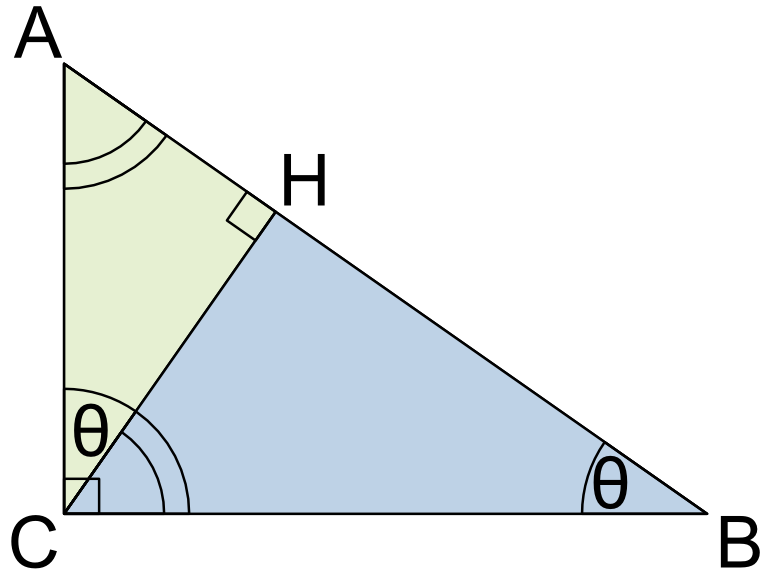
\includegraphics[width=0.3\textwidth]{figures/Pythagoras.png}
	\caption{Similar triangles used in the proof of the Pythagorean theorem.}
	\label{fig:Pythagoras}
\end{figure}

The new triangle $ACH$ is similar to triangle $ABC$, because they both have a right angle (by definition of the altitude), and they share the angle at $A$, meaning that the third angle will be the same in both triangles as well, marked as $\theta$ in Figure~\ref{fig:Pythagoras}. By a similar reasoning, the triangle $CBH$ is also similar to $ABC$. 

Similarity of the triangles leads to the equality of ratios of corresponding sides:
\begin{equation}
    \frac{BC}{AB}=\frac{BH}{BC} \text{ and } \frac{AC}{AB}=\frac{AH}{AC}.
\end{equation}
The first result equates $\cos \theta$ and the second result equates $\sin \theta$.

These ratios can be written as:
\begin{equation}
    {BC}^{2}={AB}\times {BH} \text{ and }{AC}^{2}={AB}\times {AH}.
\end{equation}
Summing these two equalities, we obtain:
\begin{equation}
    {BC}^{2}+{AC}^{2}={AB}\times {BH}+{AB}\times {AH}={AB}\times({AH}+{BH})={AB}^{2} ,
\end{equation}
which, tidying up, is the Pythagorean theorem:
\begin{equation}
    {BC}^{2}+{AC}^{2}={AB}^{2}.
\end{equation}
\end{proof}
%
\end{appendices}
%--------------------------------------------------------------------------------------------------
%
% BACK MATTER
%--------------------------------------------------------------------------------------------------
%
\backmatter
%
% References used in the thesis
\printreferences
%
% Author's bibliography
%--------------------------------------------------------------------------------------------------
% 
\chapter{Bibliography}
%--------------------------------------------------------------------------------------------------
% Enclose with refsection and use \nocite{*}, if you need to list publications not referenced in 
% the thesis:
\begin{refsection}
\nocite{*}

\section*{Publications Related to the Thesis}

All publications related to the thesis should be referenced in the text.

\defbibheading{subbibliography}{\subsection*{Journal Articles}}
\printbibliography[heading=subbibliography,env=nolabelbib,sorting=nty,keyword=myarticle]

\defbibheading{subbibliography}{\subsection*{Conference Paper}}
\printbibliography[heading=subbibliography,env=nolabelbib,sorting=nty,keyword=myconf]

\section*{Other Publications (optional)}

\dots

\end{refsection}
%
% Author's biography
%--------------------------------------------------------------------------------------------------
%
\chapter{Biography}
%--------------------------------------------------------------------------------------------------

Jan Rupnik was born in Ljubljana on 6.12.1982. 
 
Following graduation at the Faculty of Mathematics and Physics, University of Ljubljana, 
with a degree in applied mathematics (Diploma) in 2006, he was employed as a researcher 
at the Artificial Intelligence Laboratory, Jožef Stefan Institute. In 2007 he
enroled in the New Media and E-science doctoral study program at the Jožef Stefan 
International Postgraduate School in Ljubljana, Slovenia.

His research interests include Machine Learning, Data Mining, Data
Fusion, Cross-Lingual Text Mining, Predictive Analytics, Applications of Data Mining
in different domains. Most of his research work is connected to the development of
statistical methods that enable cross-modal data integration, with focus on
scalability. 

Jan Rupnik has been involved in a number of EU FP7 projects, including
SMART (Statistical Multilingual Analysis For Retrieval And Translation), XLIKE (Cross-
lingual Knowledge Extraction), EURIDICE (The Intelligent Cargo Concept in the
European Project) and SOPHOCLES (Self-Organised information PrOcessing,
CriticaLity and Emergence in multilevel Systems).
%
% Index (optional)
\printmyindex
%--------------------------------------------------------------------------------------------------
\end{document}
